\chapter{Uncertainty extrapolation for high $p_T$ Pflow jets}
\label{app:PCBTextrap}
\chapterquote{I'm all energy, no technique.}%
{Dwayne Spiteri, referring to his squash ability.}
High-$p_T$ flavour tagging uncertainties are essential for analyses involving boosted regions. At high transverse momentum, the kinematic properties and structure of jets evolve significantly --- jets become more collimated, substructure variables are altered, and the performance of flavour tagging algorithms begins to deviate from their behaviour in the lower-$p_T$ regime. Since PFlow jets combine calorimeter and tracking information, their response and tagging behaviour at high $p_T$ are sensitive to detector effects and modelling limitations that may not be fully captured by simulations. Without properly quantified uncertainties, the scale factors (SFs) applied to match data and simulation could be misestimated, directly impacting signal efficiencies and background rates in searches for boosted objects like Higgs bosons or new resonances.
\\
\\
The PCBT approach, which allows finer granularity in the $b$-tagging decision by treating the tagger output score in efficiency bins, is particularly powerful but introduces complexity in calibration. As it treats $b$-tagging as a continuous observable rather than a binary one, the uncertainties must account not just for the $b$-tag efficiency in $p_T$, but also for the shape and migration across score bins. This shape sensitivity becomes even more crucial at high $p_T$, where the tagger response may shift due to changes in the underlying jet composition or detector resolution. As a result, PCBT requires a detailed and reliable propagation of uncertainties, especially for PFlow jets, which are more sensitive to tracking performance and pileup effects --- both of which are more variable at high energies.
\\
\\
Moreover, many physics analyses using PFlow jets and PCBT are designed to explore boosted topologies, where the sensitivity relies on correctly identifying high-$p_T$ $b$-jets. In these regions, flavour tagging uncertainties often dominate the total systematic uncertainty budget. If the uncertainties in this regime are not well modelled or are overly simplified (e.g.\ due to pruning or insufficient calibration coverage), it can lead to biased estimates of signal strengths or artificial sensitivity in limits. Accurate high-$p_T$ flavour tagging uncertainties ensure robust uncertainty propagation and enable consistent treatment across different analyses, working points, and jet definitions. This is particularly important for combinations or reinterpretations that span a wide $p_T$ range and depend on the integrity of uncertainty correlations. 
\\
\\
Here, we define the high-$p_T$ uncertainty extrapolation method used in the $t\bar{t}H(b\bar{b})$ Legacy analysis as this analysis used PFlow jets and PCBT. This piece of work was done solely to improve the uncertainty handling in the high-$p_T$ resolved and boosted regions of the $t\bar{t}H(b\bar{b})$ Legacy analysis but was later implemented in a calibration data interface (CDI) for software release 21. Meaning, that any analysis, using PFlow jets and PCBT in high-$p_T$ regions, across the ATLAS collaboration would benefit from this work.

\section{Extrapolation uncertainty} \label{sec:extrap}
Flavour tagging requires the use of data-to-simulation scale factors because the performance of the tagging algorithms in Monte Carlo simulations rarely matches that observed in real data. These differences arise due to imperfect modelling  of detector responses, the complexity of hadronization processes, and various systematic effects inherent in the simulation of physics processes. By deriving scale factors that represent the ratio of the tagging efficiency in data to that in simulation, physicists can correct for these discrepancies. This calibration ensures that analyses relying on flavour tagging have accurate efficiencies and background estimates, ultimately leading to more reliable physical measurements and limits. Hence the first ingredient in our extrapolation recipe are these scale factors.
\\
\\
In order to establish the data-to-simulation scale factor for a given flavour of jet we need an abundance of events within a given $p_T$ range. For example, to generate the efficiency scale factors used in $b$-tagging, both an enriched MC sample of $t\bar{t}$ events was used and well understood reference objects to provide in-situ calibration and uncertainties. However this approach sets a limit in which the efficiency scale factors can be reliably generated as the limited data statistics means there are $p_T$ regions beyond which the data-to-simulation scale factor cannot be reliably determined.
 For $b$-tagged Pflow jets the upper limit is $p_T$ = 400 GeV, this sets an in-situ calibration threshold on $b$-jets. The calibration threshold for each flavour of jet can be seen in \ref{tab:calibration_thresholds}. The uncertainties are then extrapolated to 3 TeV.
\\
\\
In order to effectively derive accurate systematic uncertainties that assume the scale factors are constant, beyond the calibration threshold, an extrapolation method must be used. The employed flavour tagging uncertainty extrapolation method for PCBT has a heavy reliance on data-to-simulation scale factors. Lets us briefly describe the extrapolation method for Pflow b-jets, a more detailed descriptions can be found here~\cite{ATL-PHYS-PUB-2021-003}. This method can be extended to all flavours of jets and jet types and for this study is extended to $c$ and $light$ jets. This method has already been used in the high-$p_T$ uncertainty extrapolation of VR-jets\cite{Ke:2023G/}.
\\
\\
The $b$-tagging efficiency is defined as:
\begin{equation*}
    \epsilon_{b}= \frac{\# \text{of jets that are $b$-tagged} }{\text{Total \# of jets}}.
\end{equation*}
We use this to then define our data-to-simulation scale factors (SF) like so:
\begin{equation*}
    \text{SF}_{b,w}= \frac{\epsilon^{\text{data}}_{b,w}}{\epsilon^{\text{MC}}_{b,w}},
\end{equation*}
where $\epsilon^{\text{data}}_{b,w}$ and $\epsilon^{\text{MC}}_{b,w}$ represent the efficiency obtained by data and simulation, respectively. the sub-script of $b,w$ represent the flavour and working point (60\%, 70\%, 77\%, 85\% and 100\%), respectively. 
\\
\\
In principle if we sum the efficiencies for a particular flavour in a single $p_T$ bin across all working points, we should reach a closure point of 1, for this example we will assume a $b$-jet using one working point to simplify the notation:
\begin{equation**}
    \sum_{i} \epsilon^{i}_{p_T} = 1.
\end{equation**}
However, approaching and beyond the calibration threshold of a particular flavour, the closure is not achieved. We introduce the data-to-simulation scale factor in-order to correct the efficiency, but closure is still not met:
\begin{equation**}
    \sum_{i} \epsilon^{i}_{p_T} \text{SF}^{i}_{p_T} = 1.
\end{equation**}
Attempting to bring us closer to closure, we proceed to expand the scale factor to include the relative scale factor corrected efficiency, $\Delta_{rel} \text{SF}_{p_T}$:
\begin{equation**}
    \sum_{i} \epsilon^{i}_{p_T} \text{SF}^{i}_{p_T} (1-\Delta_{rel} \text{SF}_{p_T}) = 1.
\end{equation**}
Expanding $\Delta_{rel} \text{SF}_{p_T}$ we find:
\begin{equation}
     \Delta_{rel}(\text{SF}_{pt})=\Delta_{rel}(\text{SF}_{pt,ref})+\Delta_{ref}(\epsilon_{MC,pt})-\Delta_{ref}(\epsilon_{MC,pt,ref}),
        \label{eq:extrapolation}
\end{equation}
where, $\Delta_{rel}(\text{SF}_{pt,ref})$ is the in-situ calibration SF relative uncertainty at the calibration threshold $p_T$ for our desired flavour and $\Delta_{ref}(\epsilon_{MC,pt})-\Delta_{ref}(\epsilon_{MC,pt,ref})$ is our extrapolation uncertainty which is purely based on simulation (this object is plotted in Figures \ref{fig:trackextrap}, \ref{fig:jetextrap}, \ref{fig:modelextrap} and \ref{fig:globalextrap}, for our tracking, jet calibration, modeling and global extrapolation uncertainty respectively.) and contains the simulation efficiency evaluated at our desired $p_T$ and the simulation efficiency at our calibration threshold $p_T$, respectively. 

\begin{table}
    \centering
    \begin{tabular}{|c|c|}\hline
         Flavour&  Calibration threshold (GeV)\\\hline
         $b$&  400\\\hline
         $c$&  250\\\hline
         $light$&  300\\ \hline
    \end{tabular}
    \caption{Caption}
    \label{tab:calibration_thresholds}
\end{table}
\\
\\
For our desired flavour of Pflow jet we need use the extrapolation uncertainty contained in Eq.~\ref{eq:extrapolation} and extrapolate all systematic uncertainties to evaluate them past the calibration threshold. The following plots are for $b$-jets at a 60\% WP and generated using Z' samples, which is a MC sample that is enriched with $t\bar{t}$ events in order to effectively evaluate the SFs at their desired $p_T$ beyond any calibration threshold. 

\subsection{Tracking uncertainties}\label{sec:trackunc}
As we see in Figures~\ref{fig:track} and~\ref{fig:trackextrap}, the relative tracking uncertainties and tracking extrapolation uncertainties respectively, the contributions to the overall extrapolation tracking uncertainty are minimal, peaking at $\approx$ 0.03 at 3 TeV.
\begin{figure}[htbp]
    \centering
    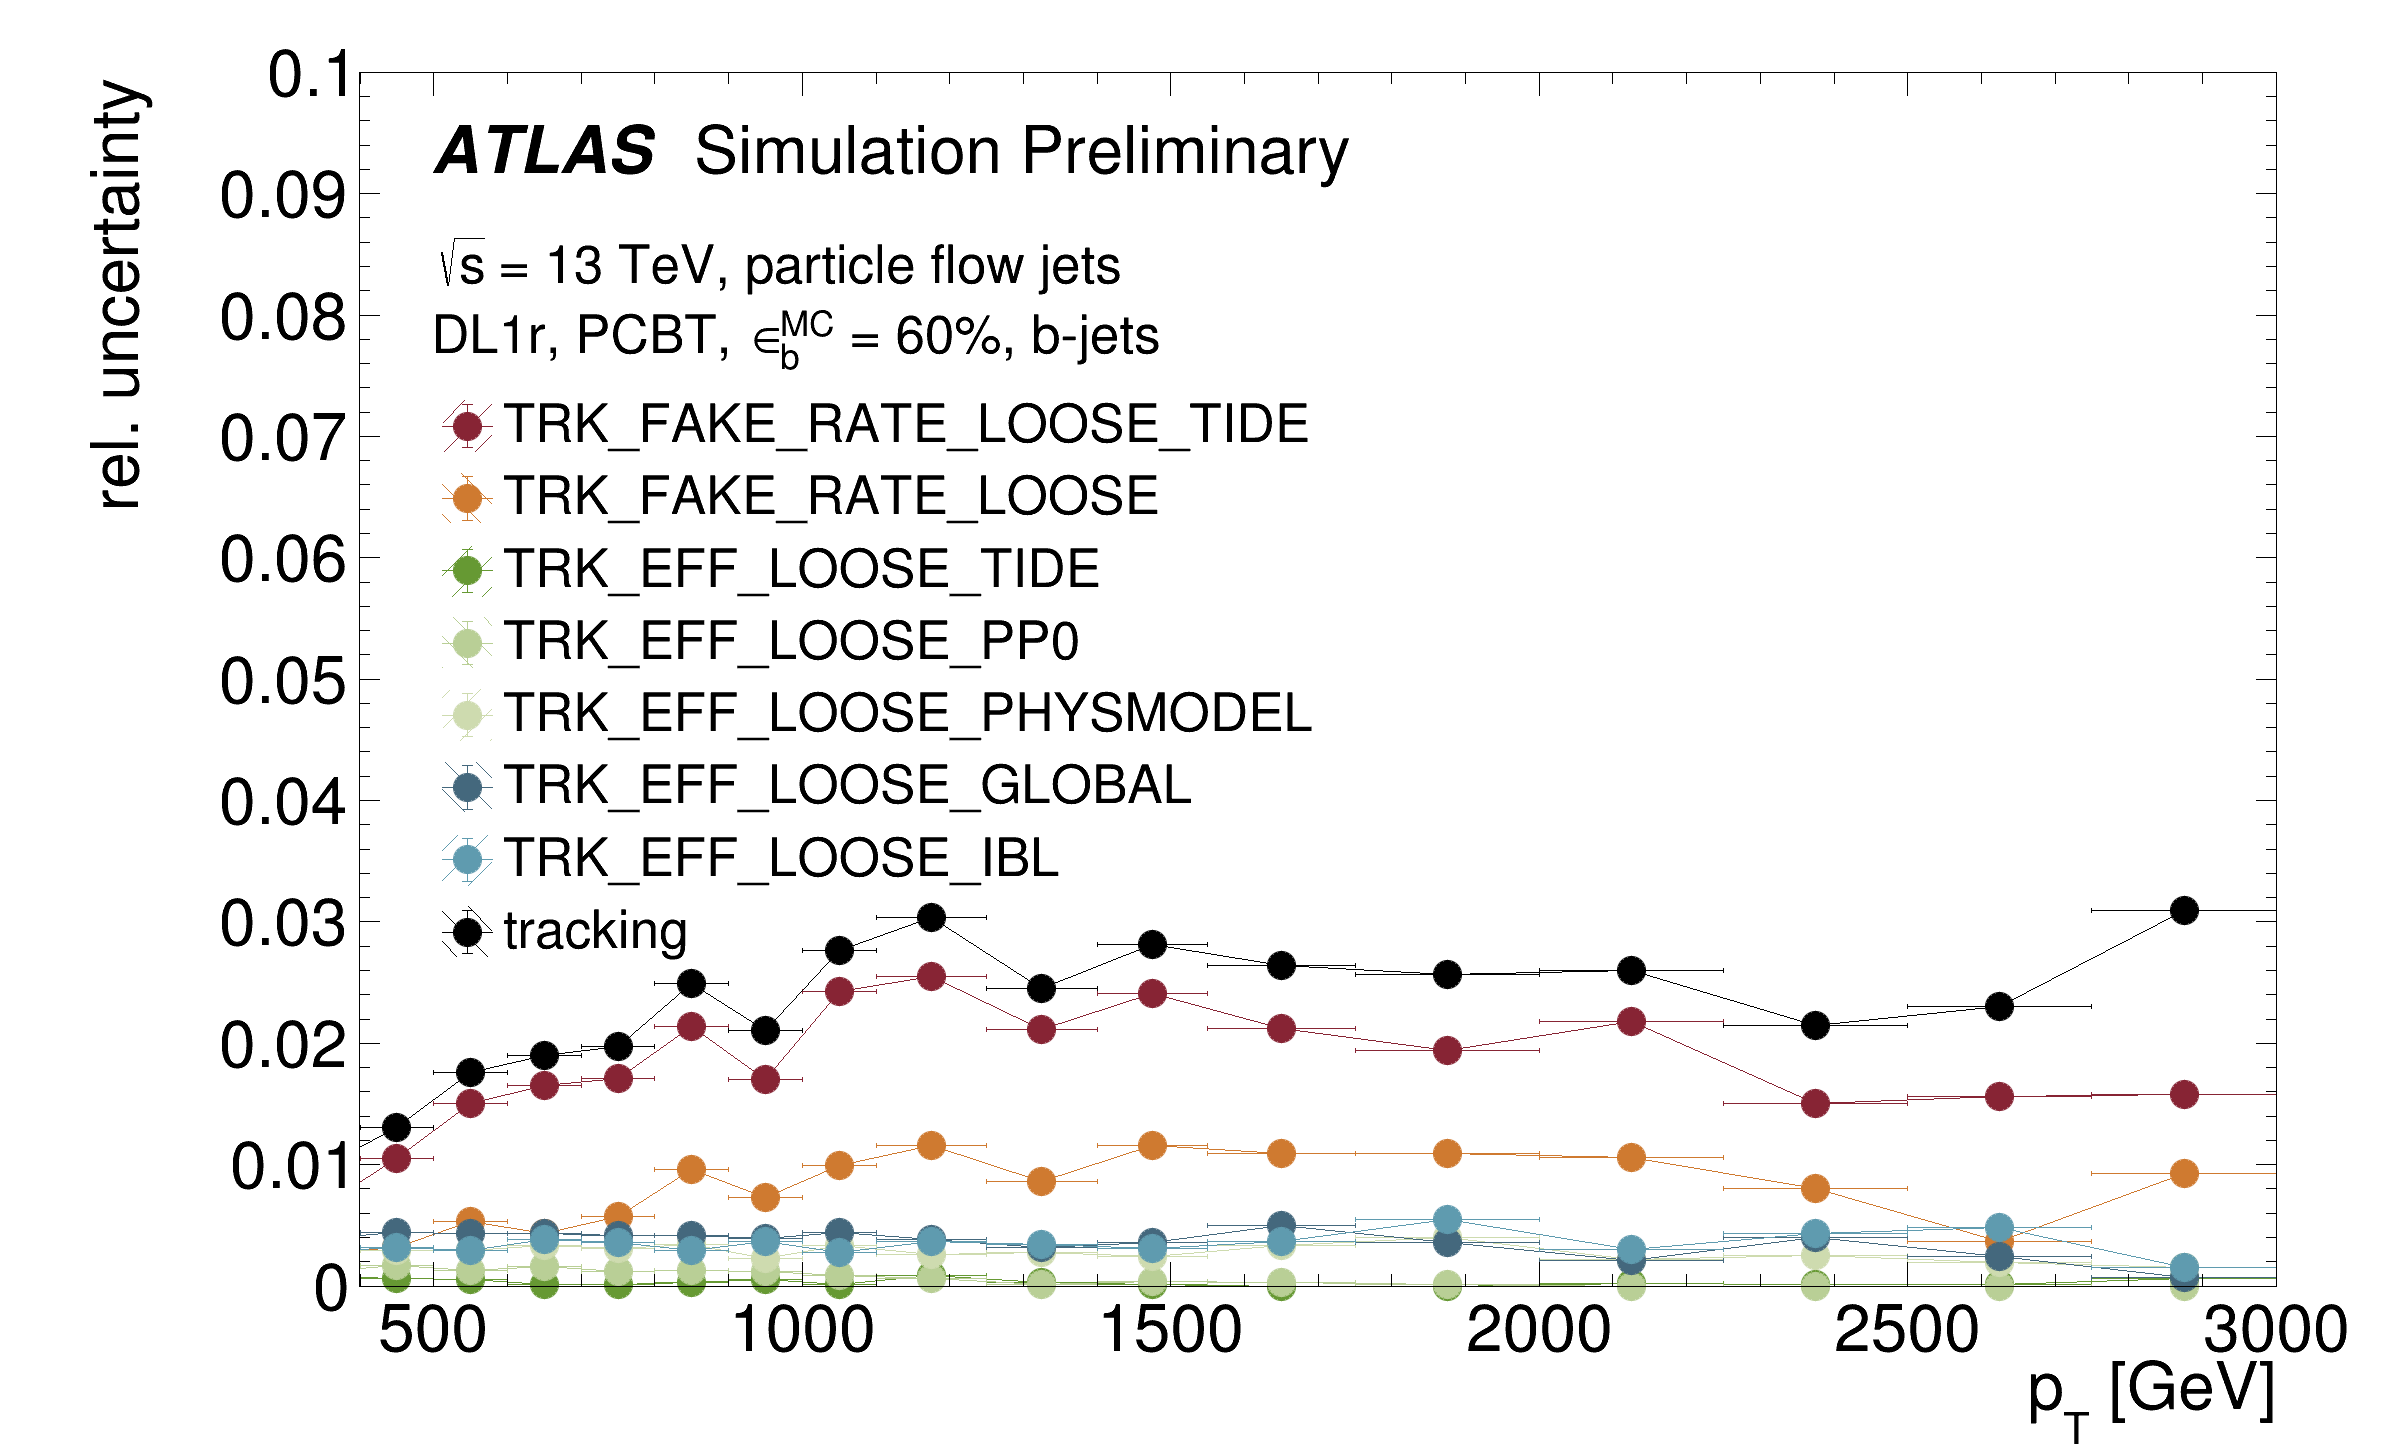
\includegraphics[scale=0.15]{figures/App_btag_highpt_extrap/tracking_detailed_1_uncs__1_.png}
    \caption{The decomposed tracking uncertainty containing: the loose tracking fake rate both in and out of a dense environment (red and orange respectively), the tracking efficiency in a dense environment (dark green), the loose tracking efficiency of the primary particles at the interaction point (light green) the loose tracking efficiency of the physical model being tested, the loose global tracking efficiency (dark blue), the loose tracking efficiency of the insertable B-layer and the combination of all tracking uncertainties (black).}
        \label{fig:track}
\end{figure}


\begin{figure}[htbp]
    \centering
    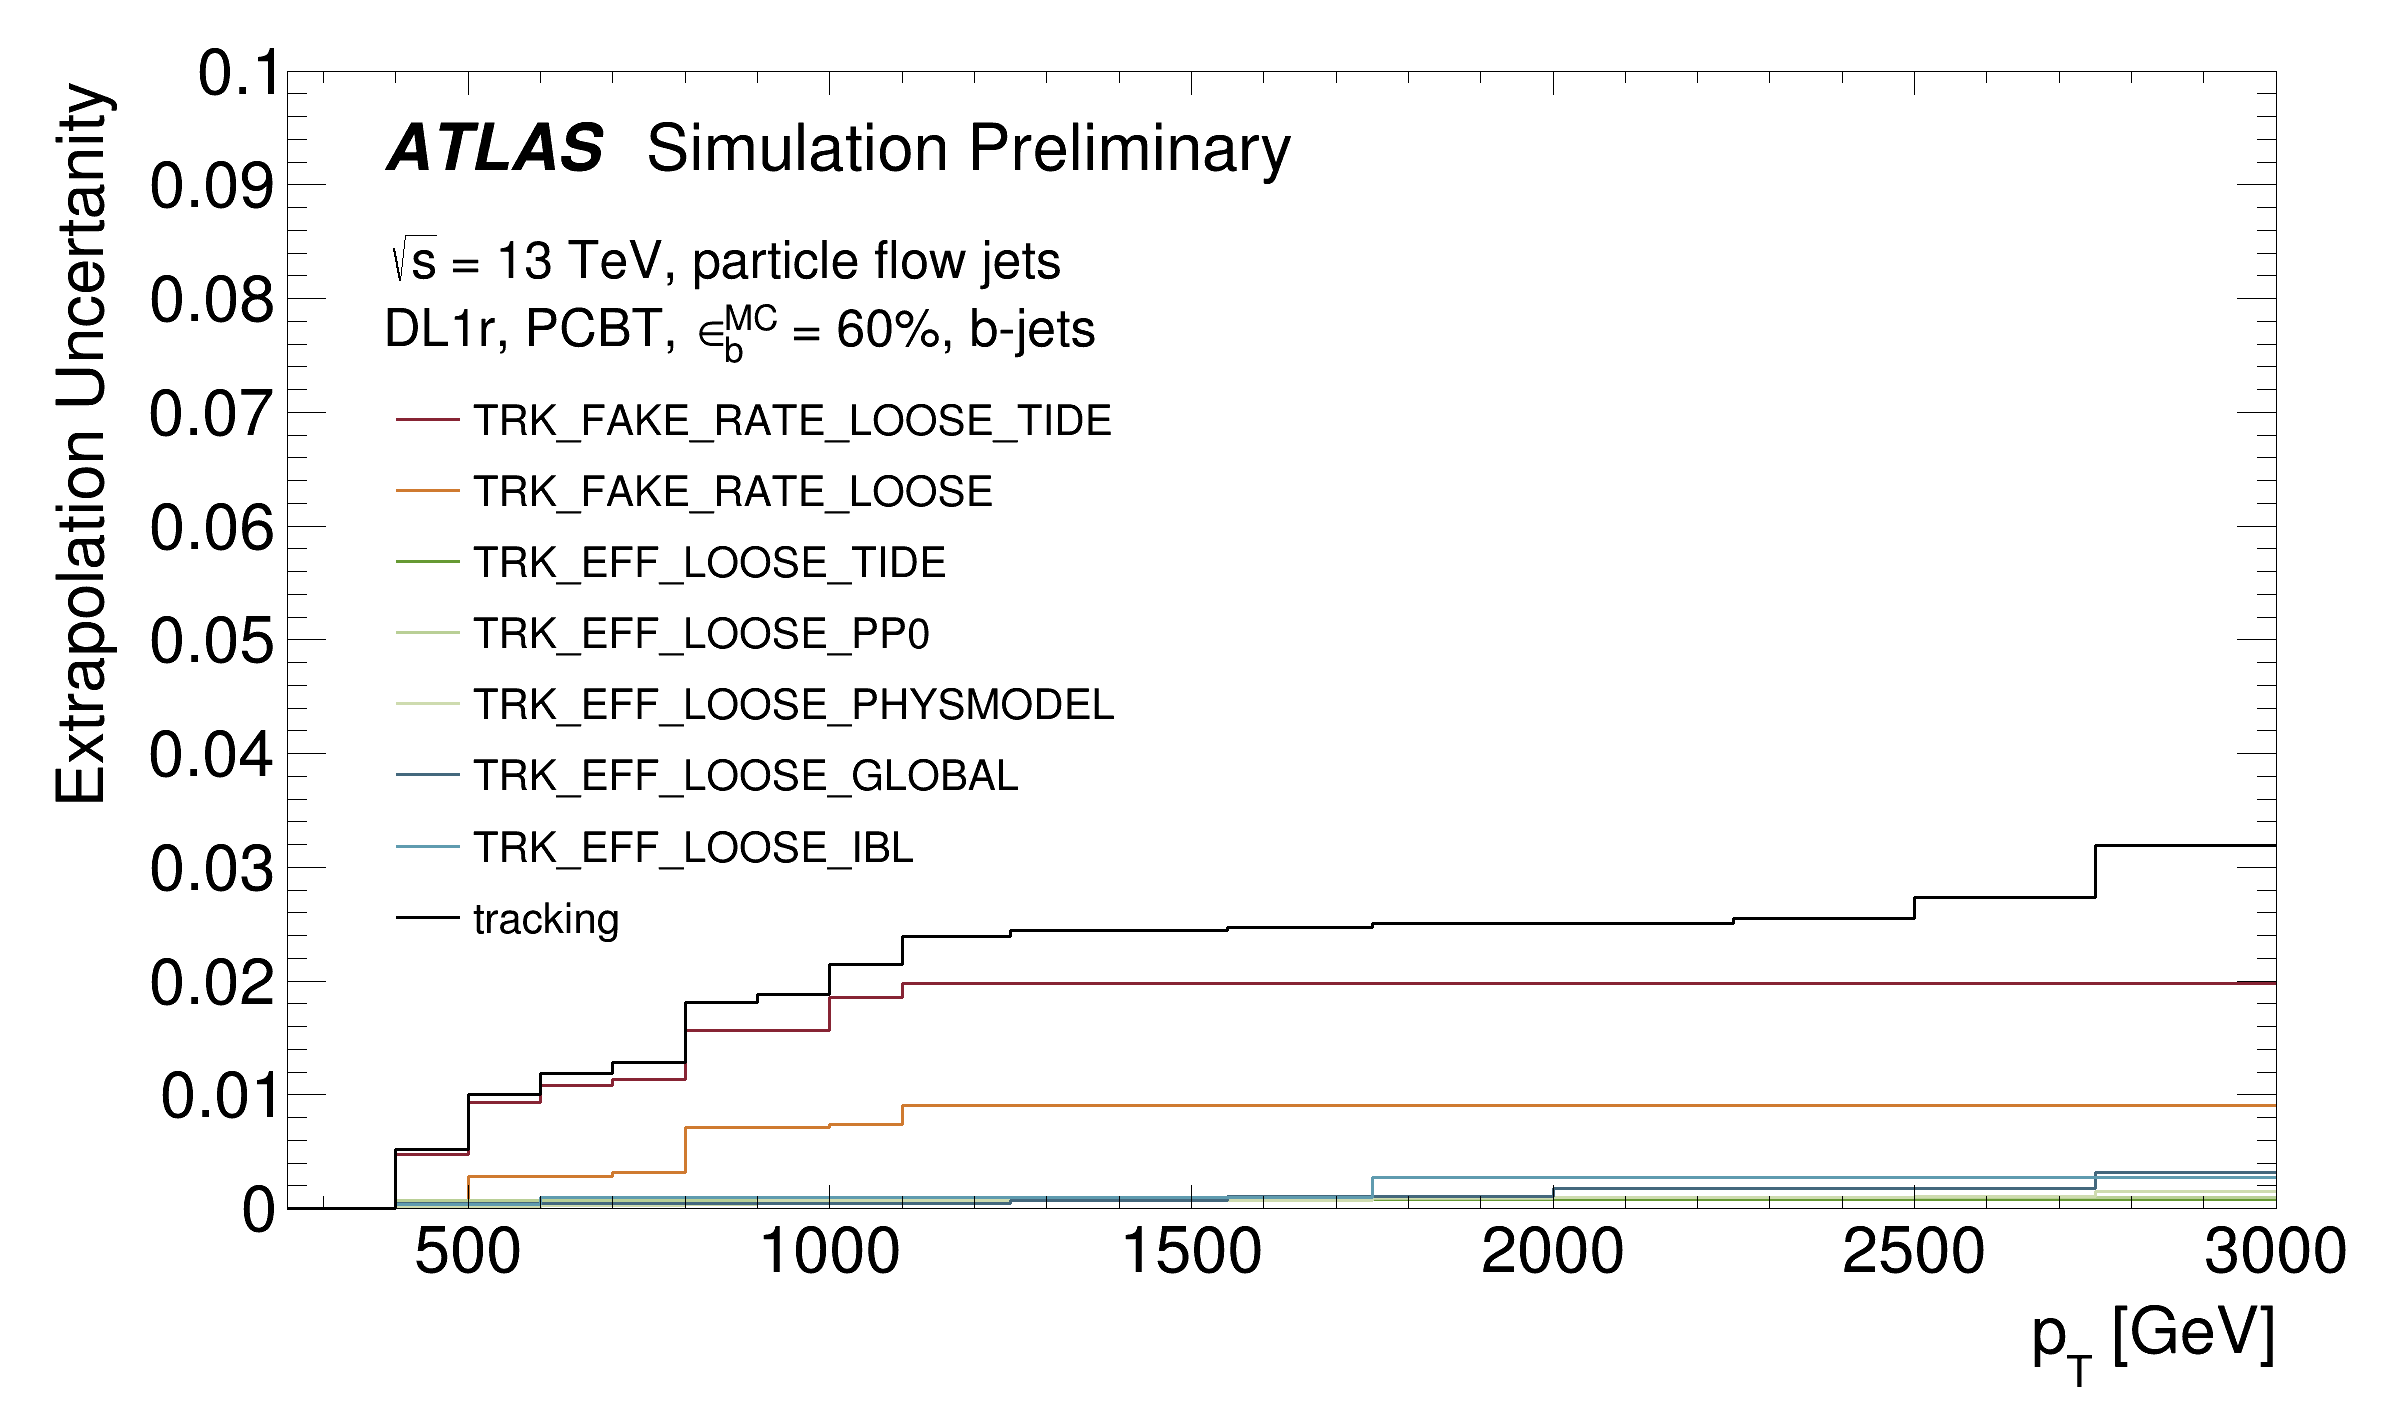
\includegraphics[scale=0.15]{figures/App_btag_highpt_extrap/tracking_detailed_1_extrap_uncs.png}
    \caption{The tracking extrapolation uncertainty containing: the loose tracking fake rate both in and out of a dense environment (red and orange respectively), the tracking efficiency in a dense environment (dark green), the loose tacking efficiency of the primary particles at the interaction point (light green) the loose tracking efficiency of the physical model being tested, the loose global tracking efficiency (dark blue), the loose tracking efficiency of the insertable B-layer and the combination of all tracking uncertainties (black).}
        \label{fig:trackextrap}
\end{figure}


\subsection{Jet calibration uncertainties} \label{sec:jetcalunc}

Much like the tracking uncertainties, the jet calibration and jet calibration extrapolation uncertainties show in Figures \ref{fig:jetcal} and \ref{fig:jetextrap}, respectively, are similarly quite minimal. The peak of the distribution seen to be $\approx$ 0.05 at 3 TeV. 

\begin{figure}[htbp]
    \centering
    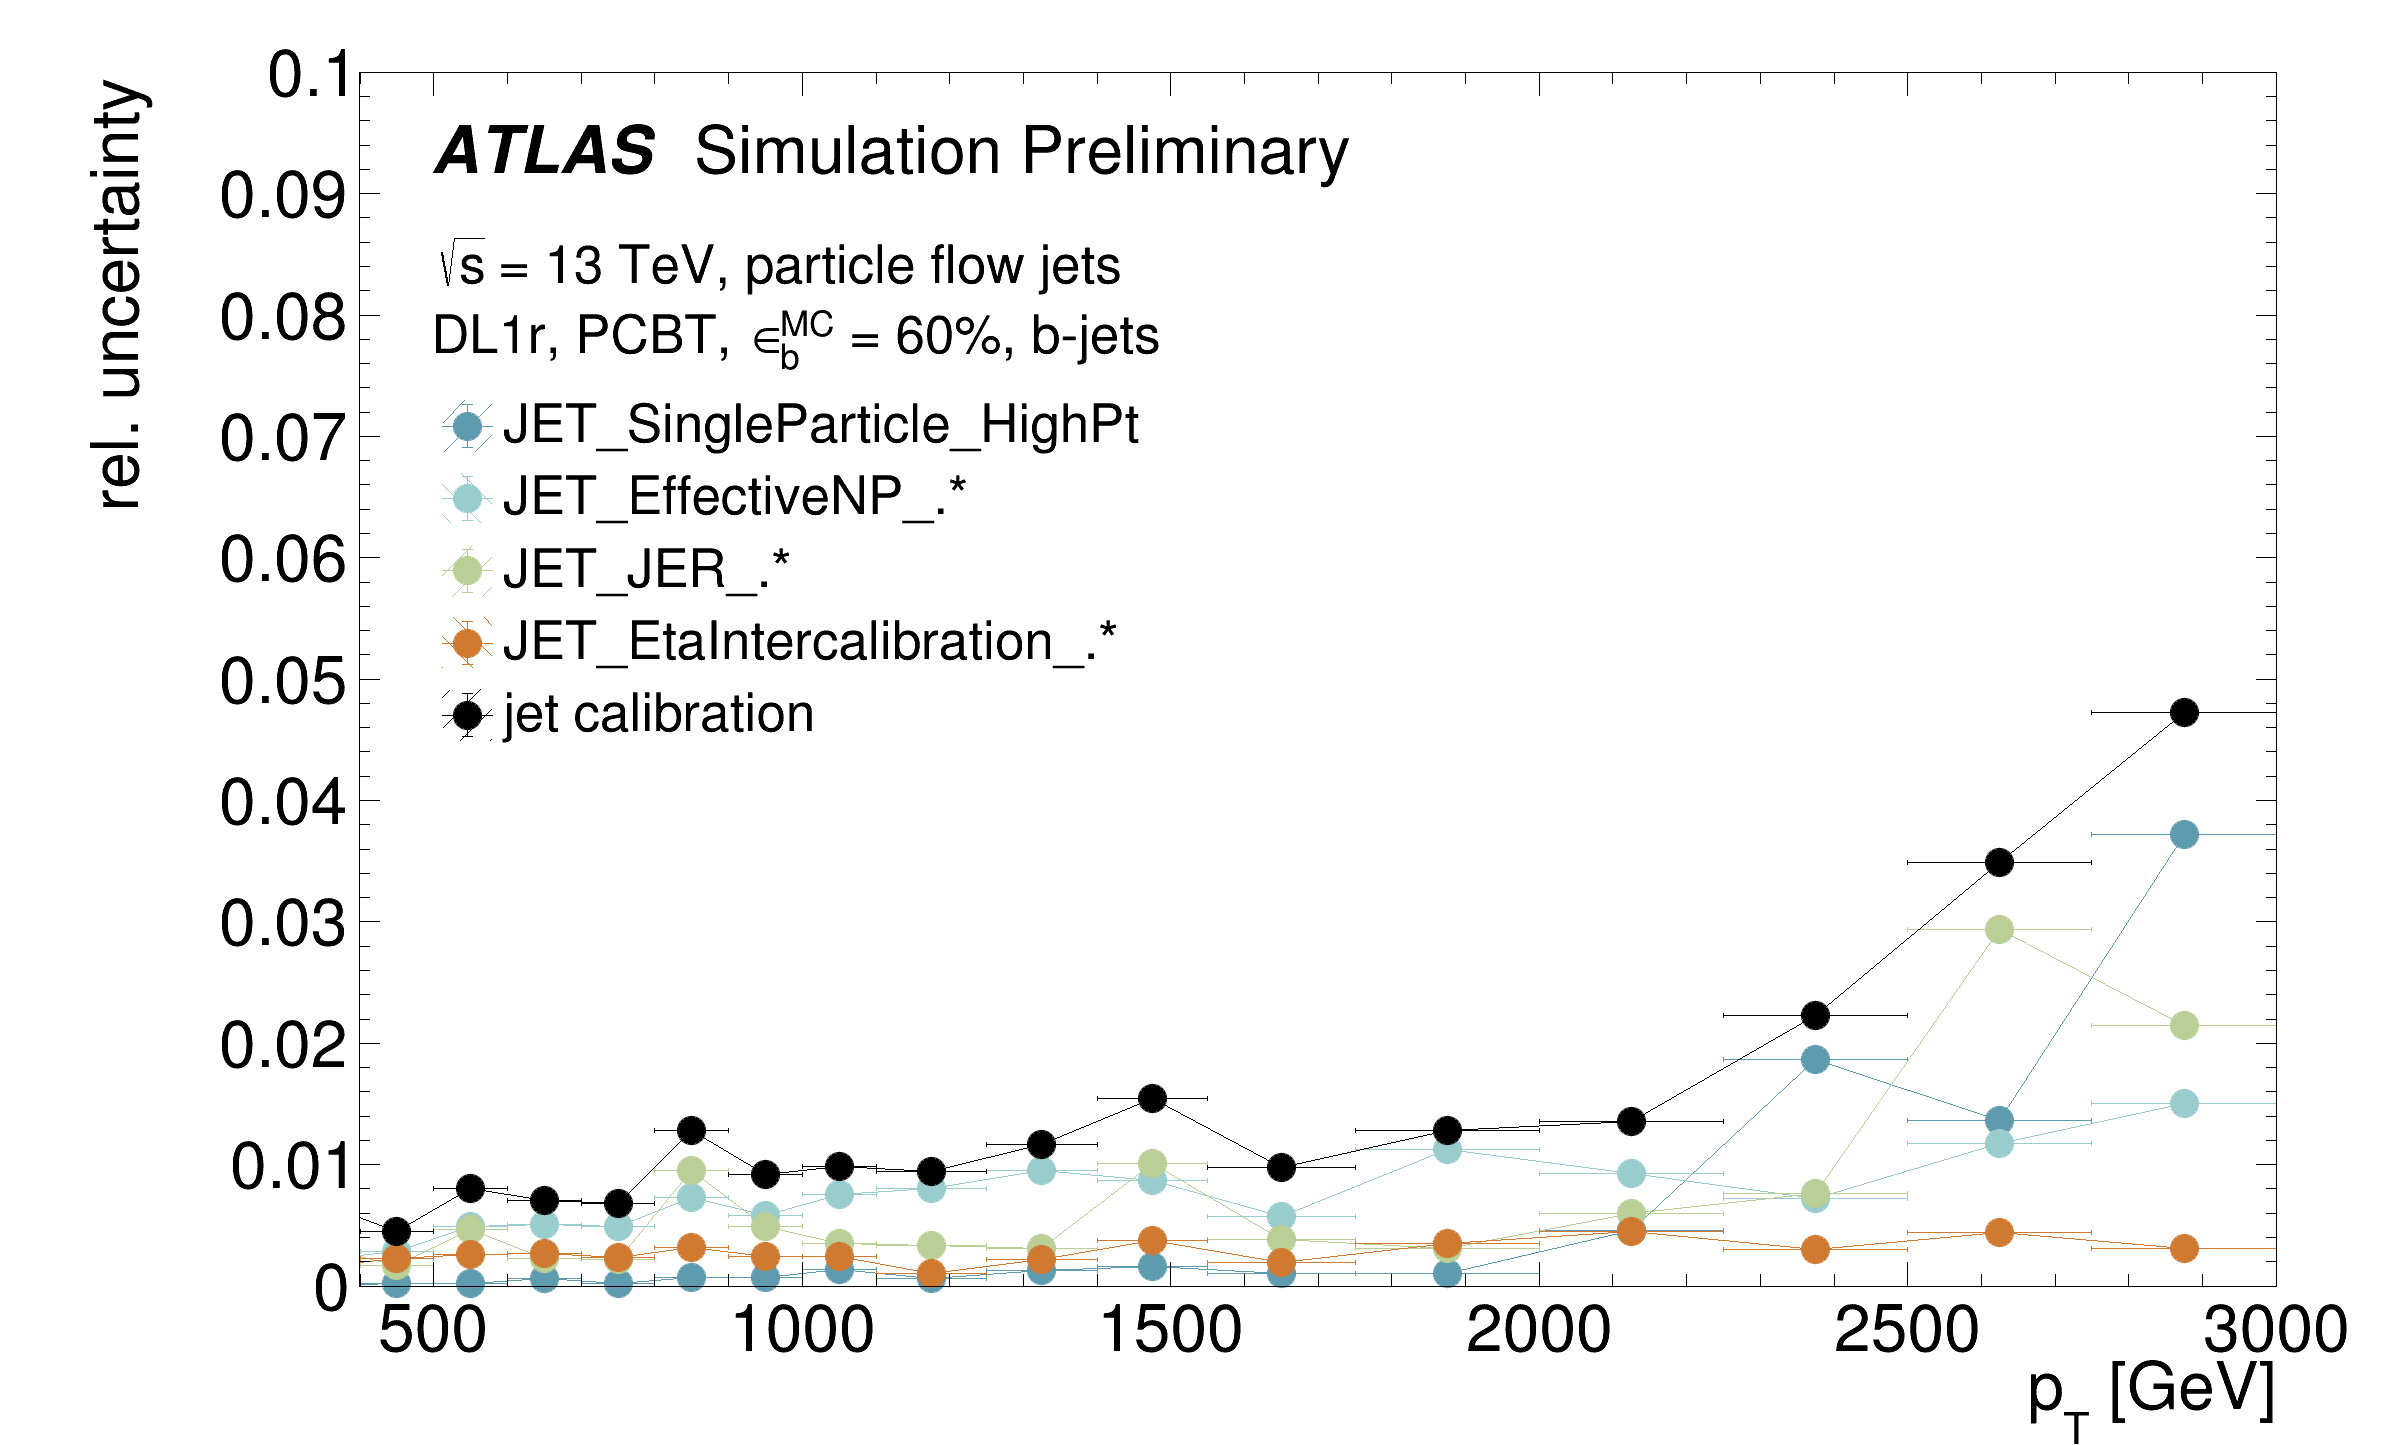
\includegraphics[scale=0.15]{figures/App_btag_highpt_extrap/jet_detailed_1_uncs__1_.png}
    \caption{The decomposed jet calibration uncertainty containing: The single particle at high $p_T$ (dark blue), the effective nuisance parameters (light blue) which is defined as the compressed representation of the full set of JES uncertainty components. JER, the jet eta inter calibrating (orange) and the combination of all jet calibration uncertainties (black)  }
        \label{fig:jetcal}
\end{figure}


\begin{figure}[htbp]
    \centering
    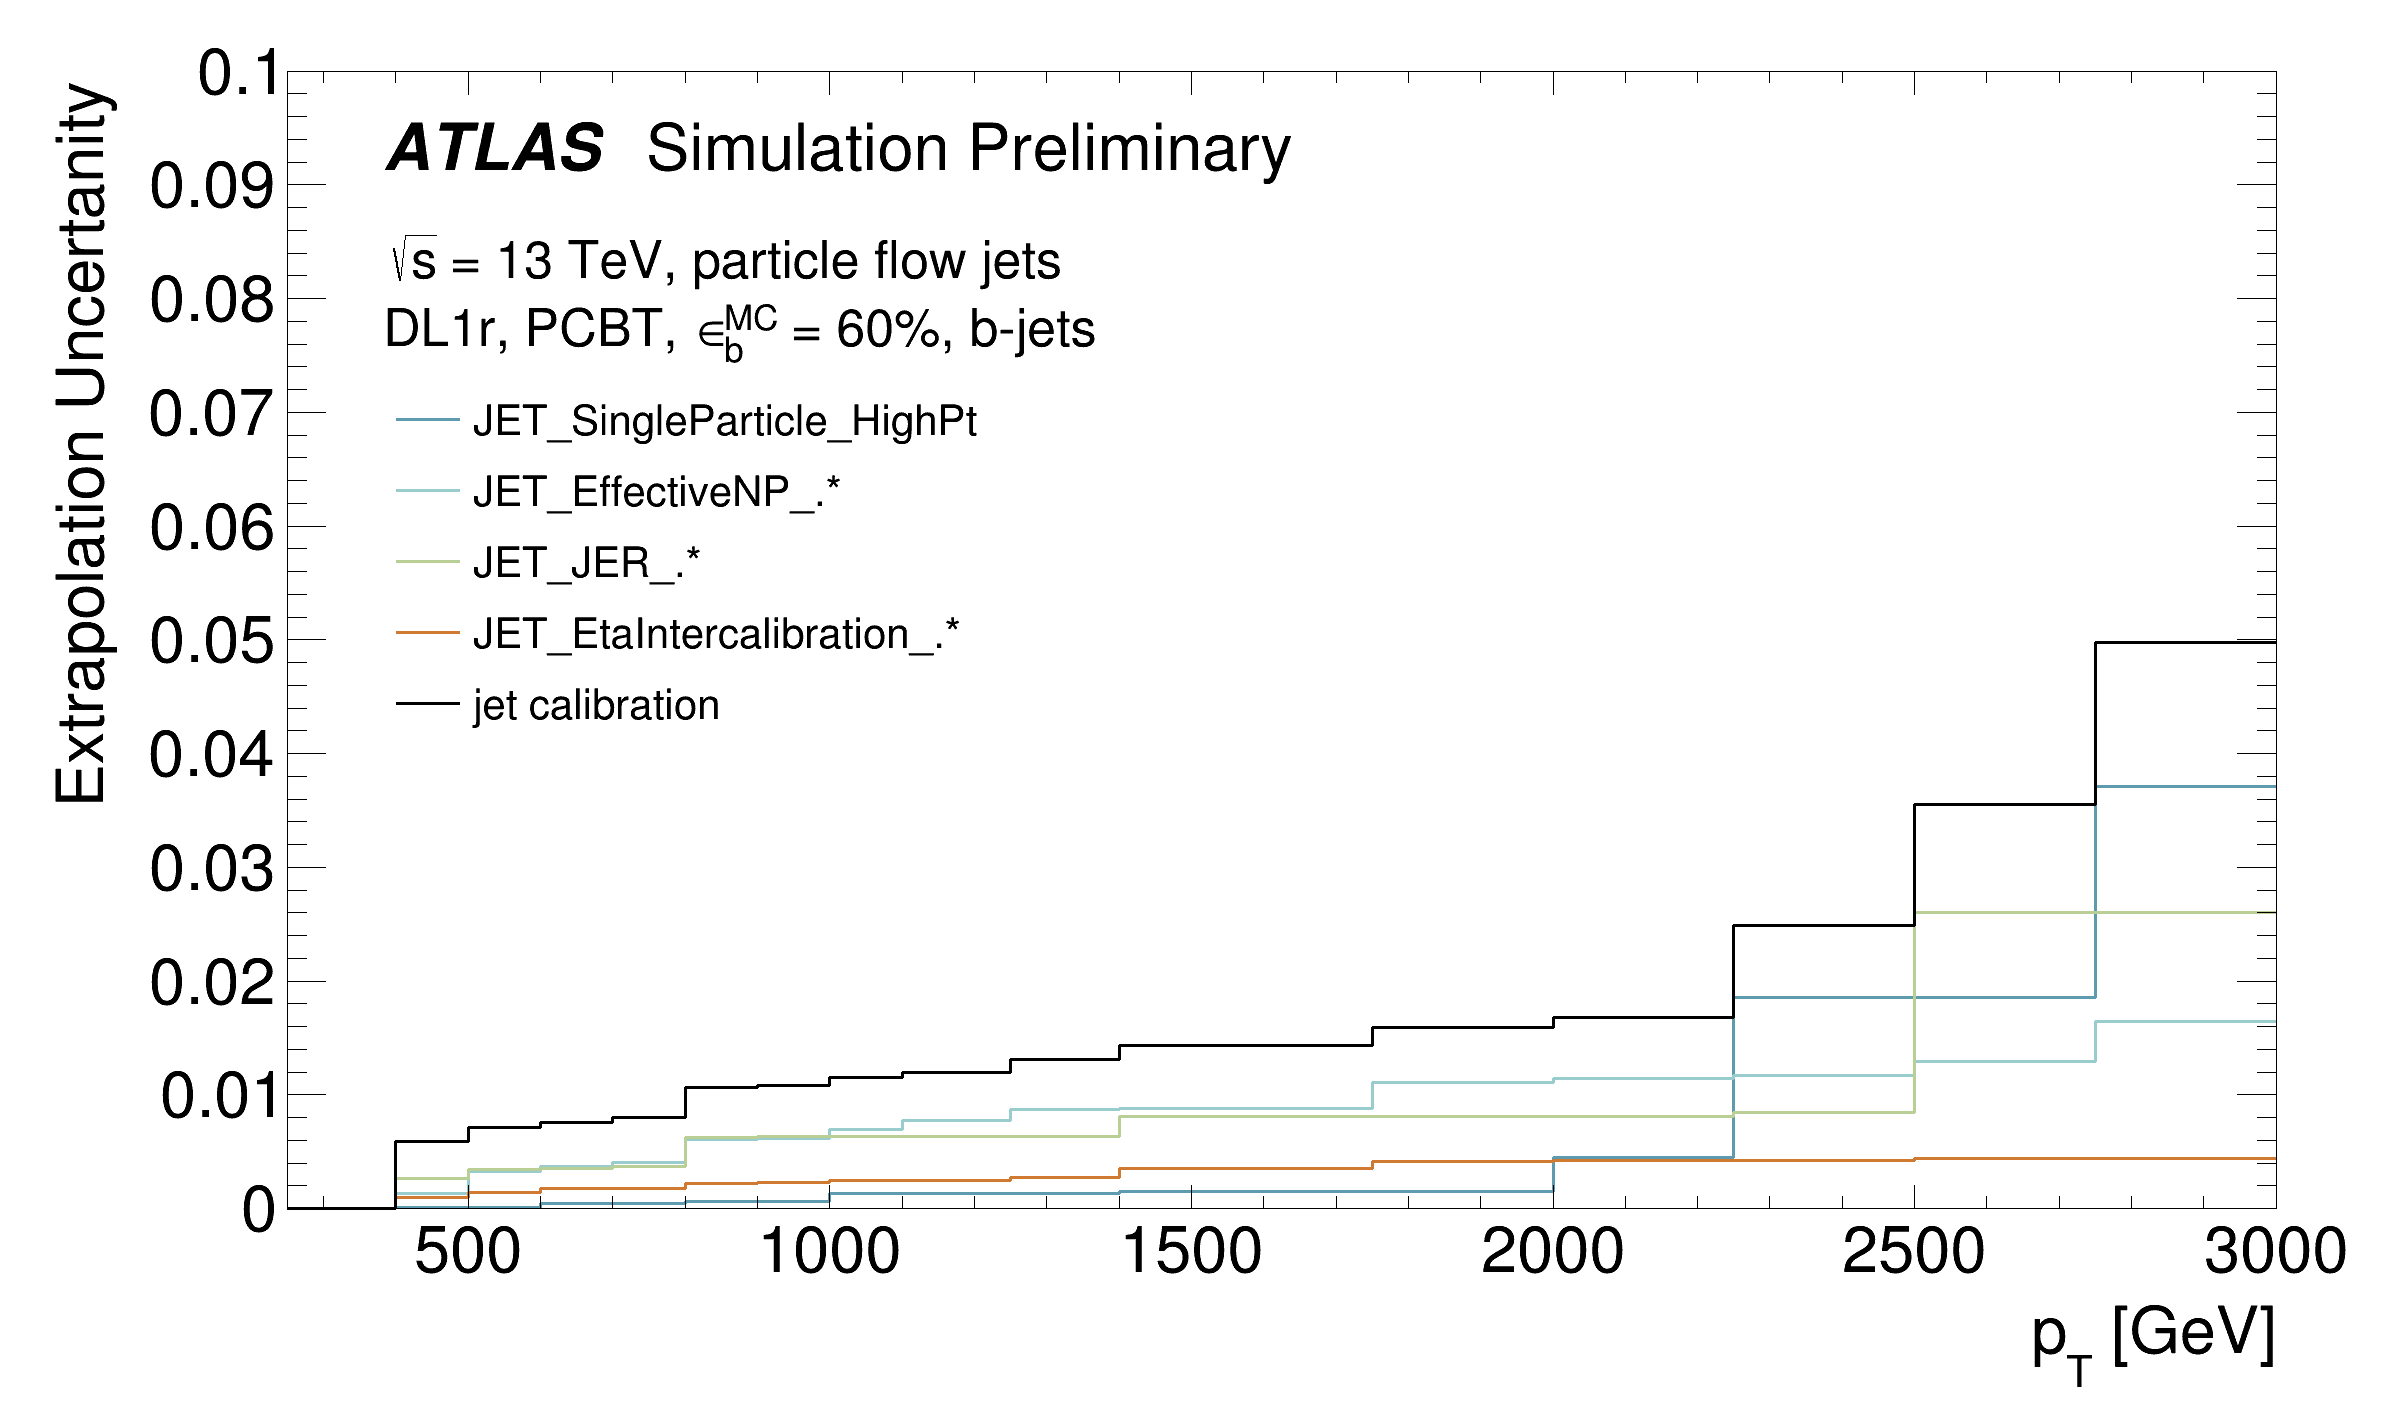
\includegraphics[scale=0.15]{figures/App_btag_highpt_extrap/jet_detailed_1_extrap_uncs.png}
    \caption{The jet calibration extrapolation uncertainty containing: The single particle at high $p_T$ (dark blue), the effective nuisance parameters (light blue). JER, the jet eta inter calibrating (orange) and the combination of all jet calibration uncertainties (black) }
        \label{fig:jetextrap}
\end{figure}

\subsection{Modeling uncertainties} \label{sec:model}

Compared to the systematics described in Sections~\ref{sec:trackunc} and~\ref{sec:jetcalunc} the modeling uncertainties are considerably higher as seen in Figure~\ref{fig:model}. With the main contributions coming from the parton shower and B-hadron interactions. When these are propagated in to the extrapolation uncertainty, as shown in Figure~\ref{fig:modelextrap}, these significantly inflate the overall value at any $p_T$ bin, peaking at 0.36 at 3 TeV.
\begin{figure}[htbp]
    \centering
    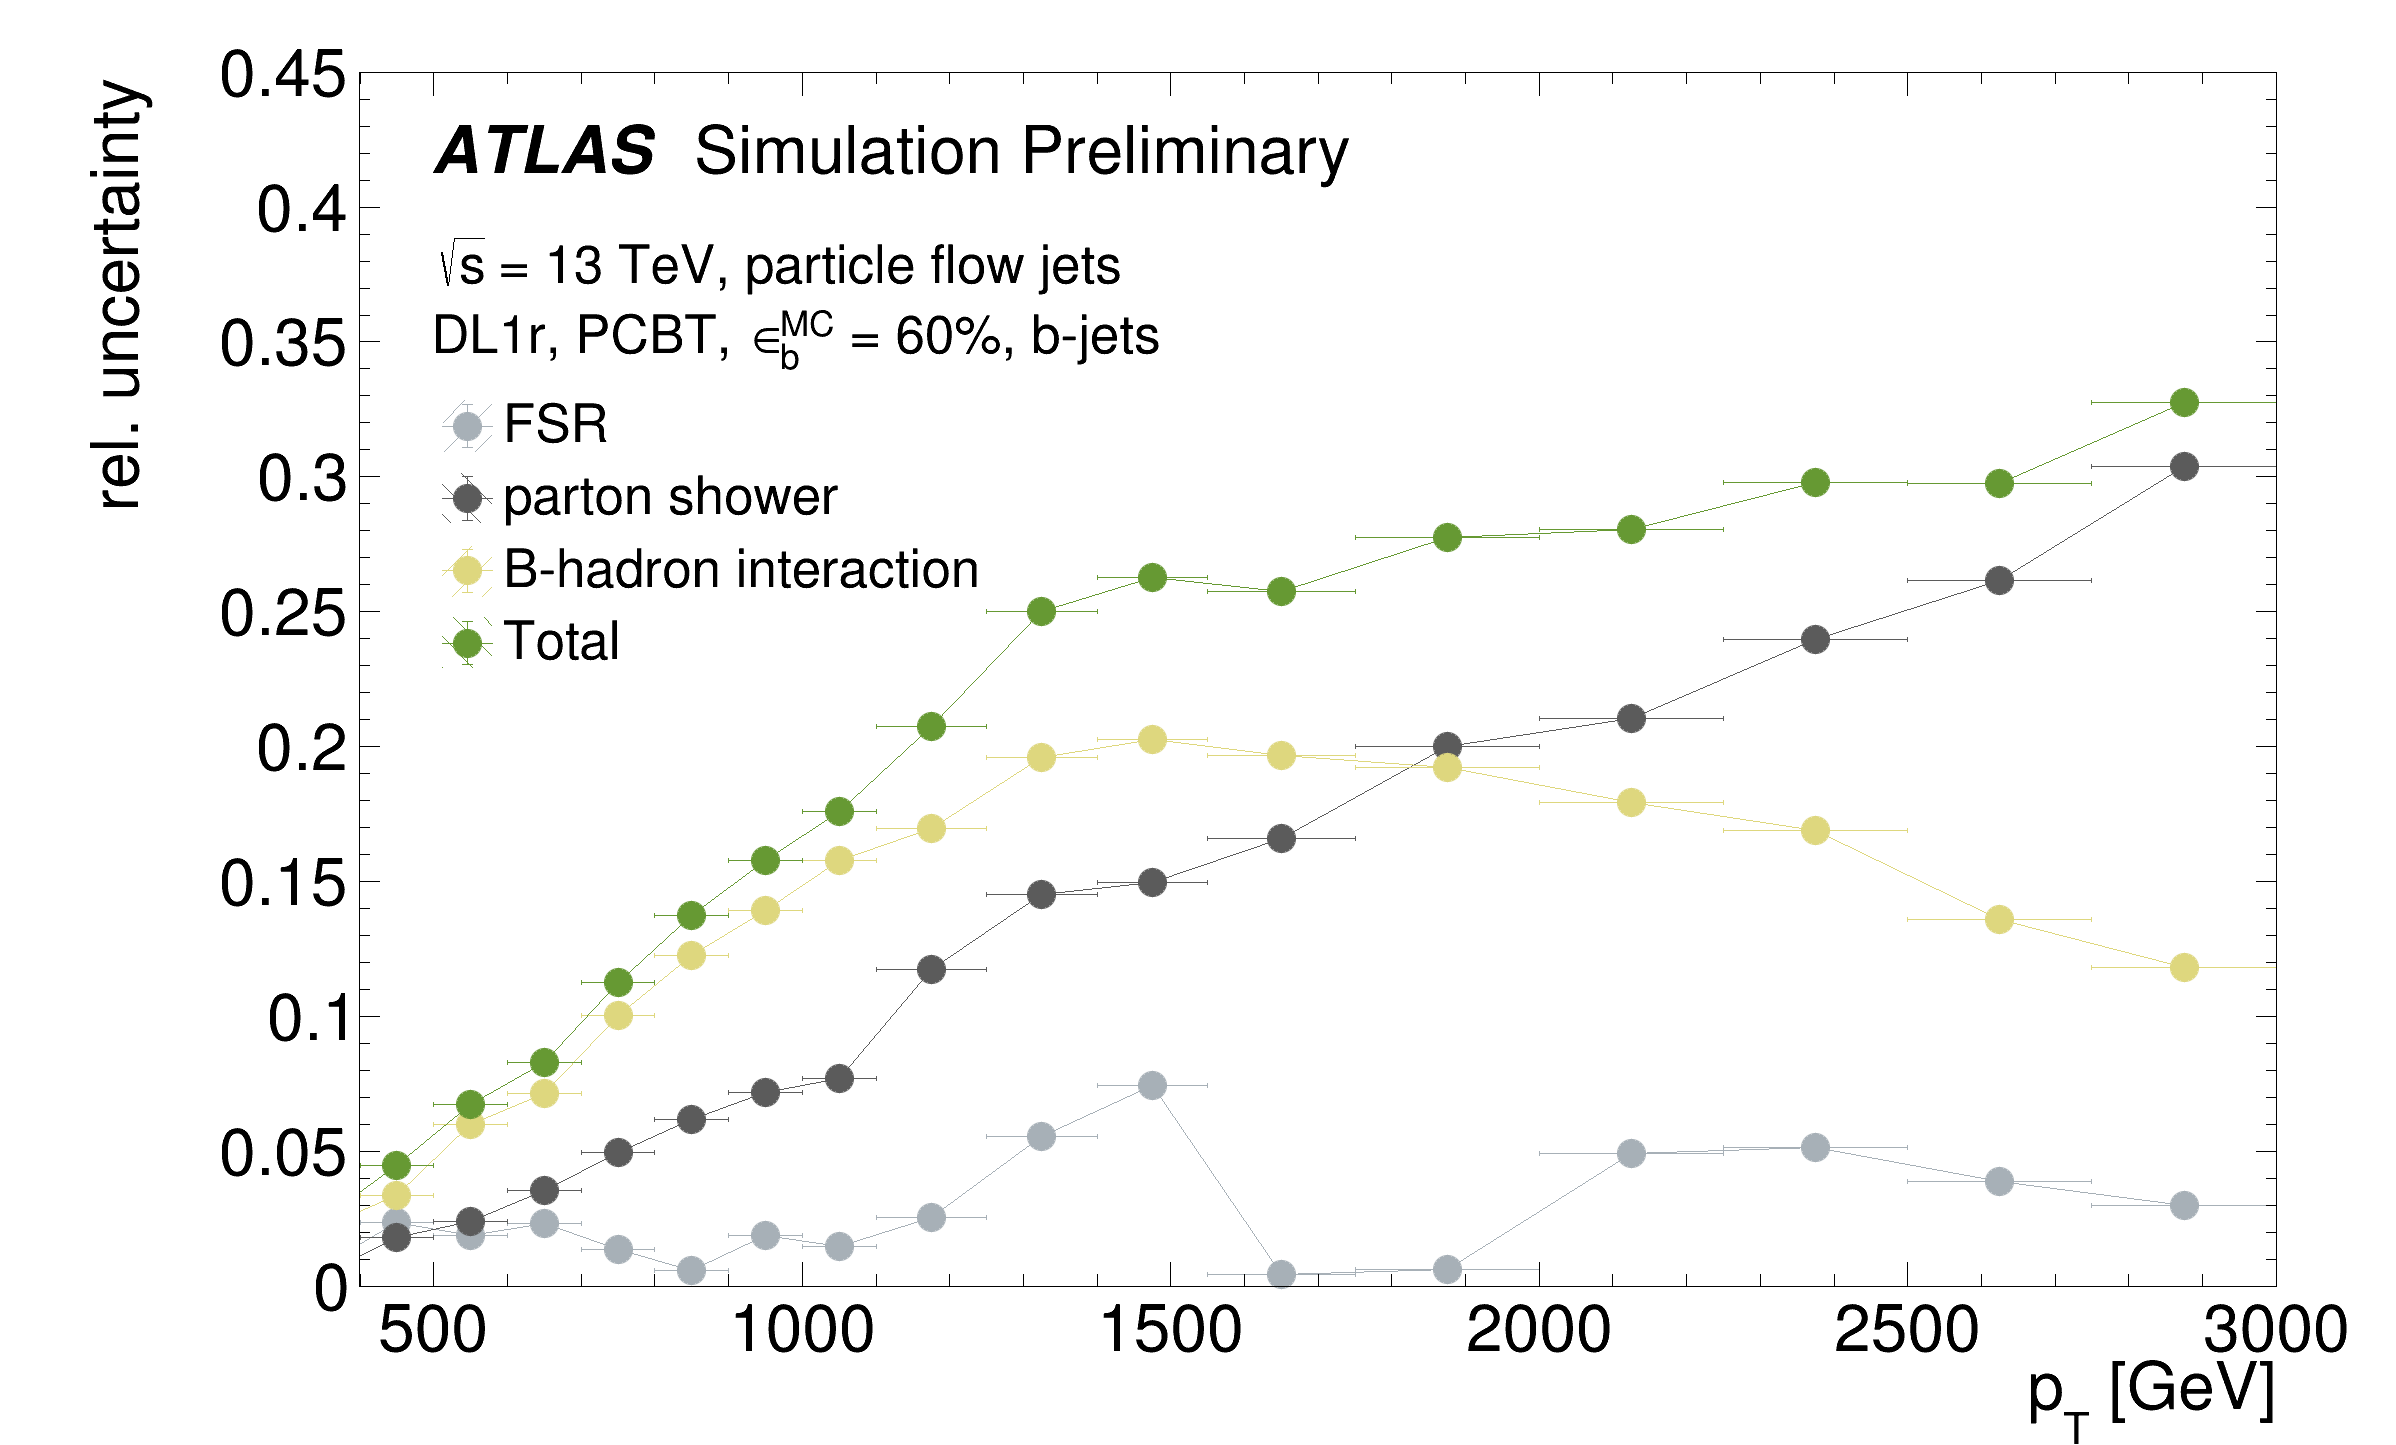
\includegraphics[scale=0.15]{figures/App_btag_highpt_extrap/modelling_important_uncs.png}
    \caption{The decomposed modeling uncertainty containing: Final state radiation (FSR, light grey), B-hadron interaction (yellow), parton shower (dark grey) and the total combination of all modeling systematics (green). }
        \label{fig:model}
\end{figure}


\begin{figure}[htbp]
    \centering
    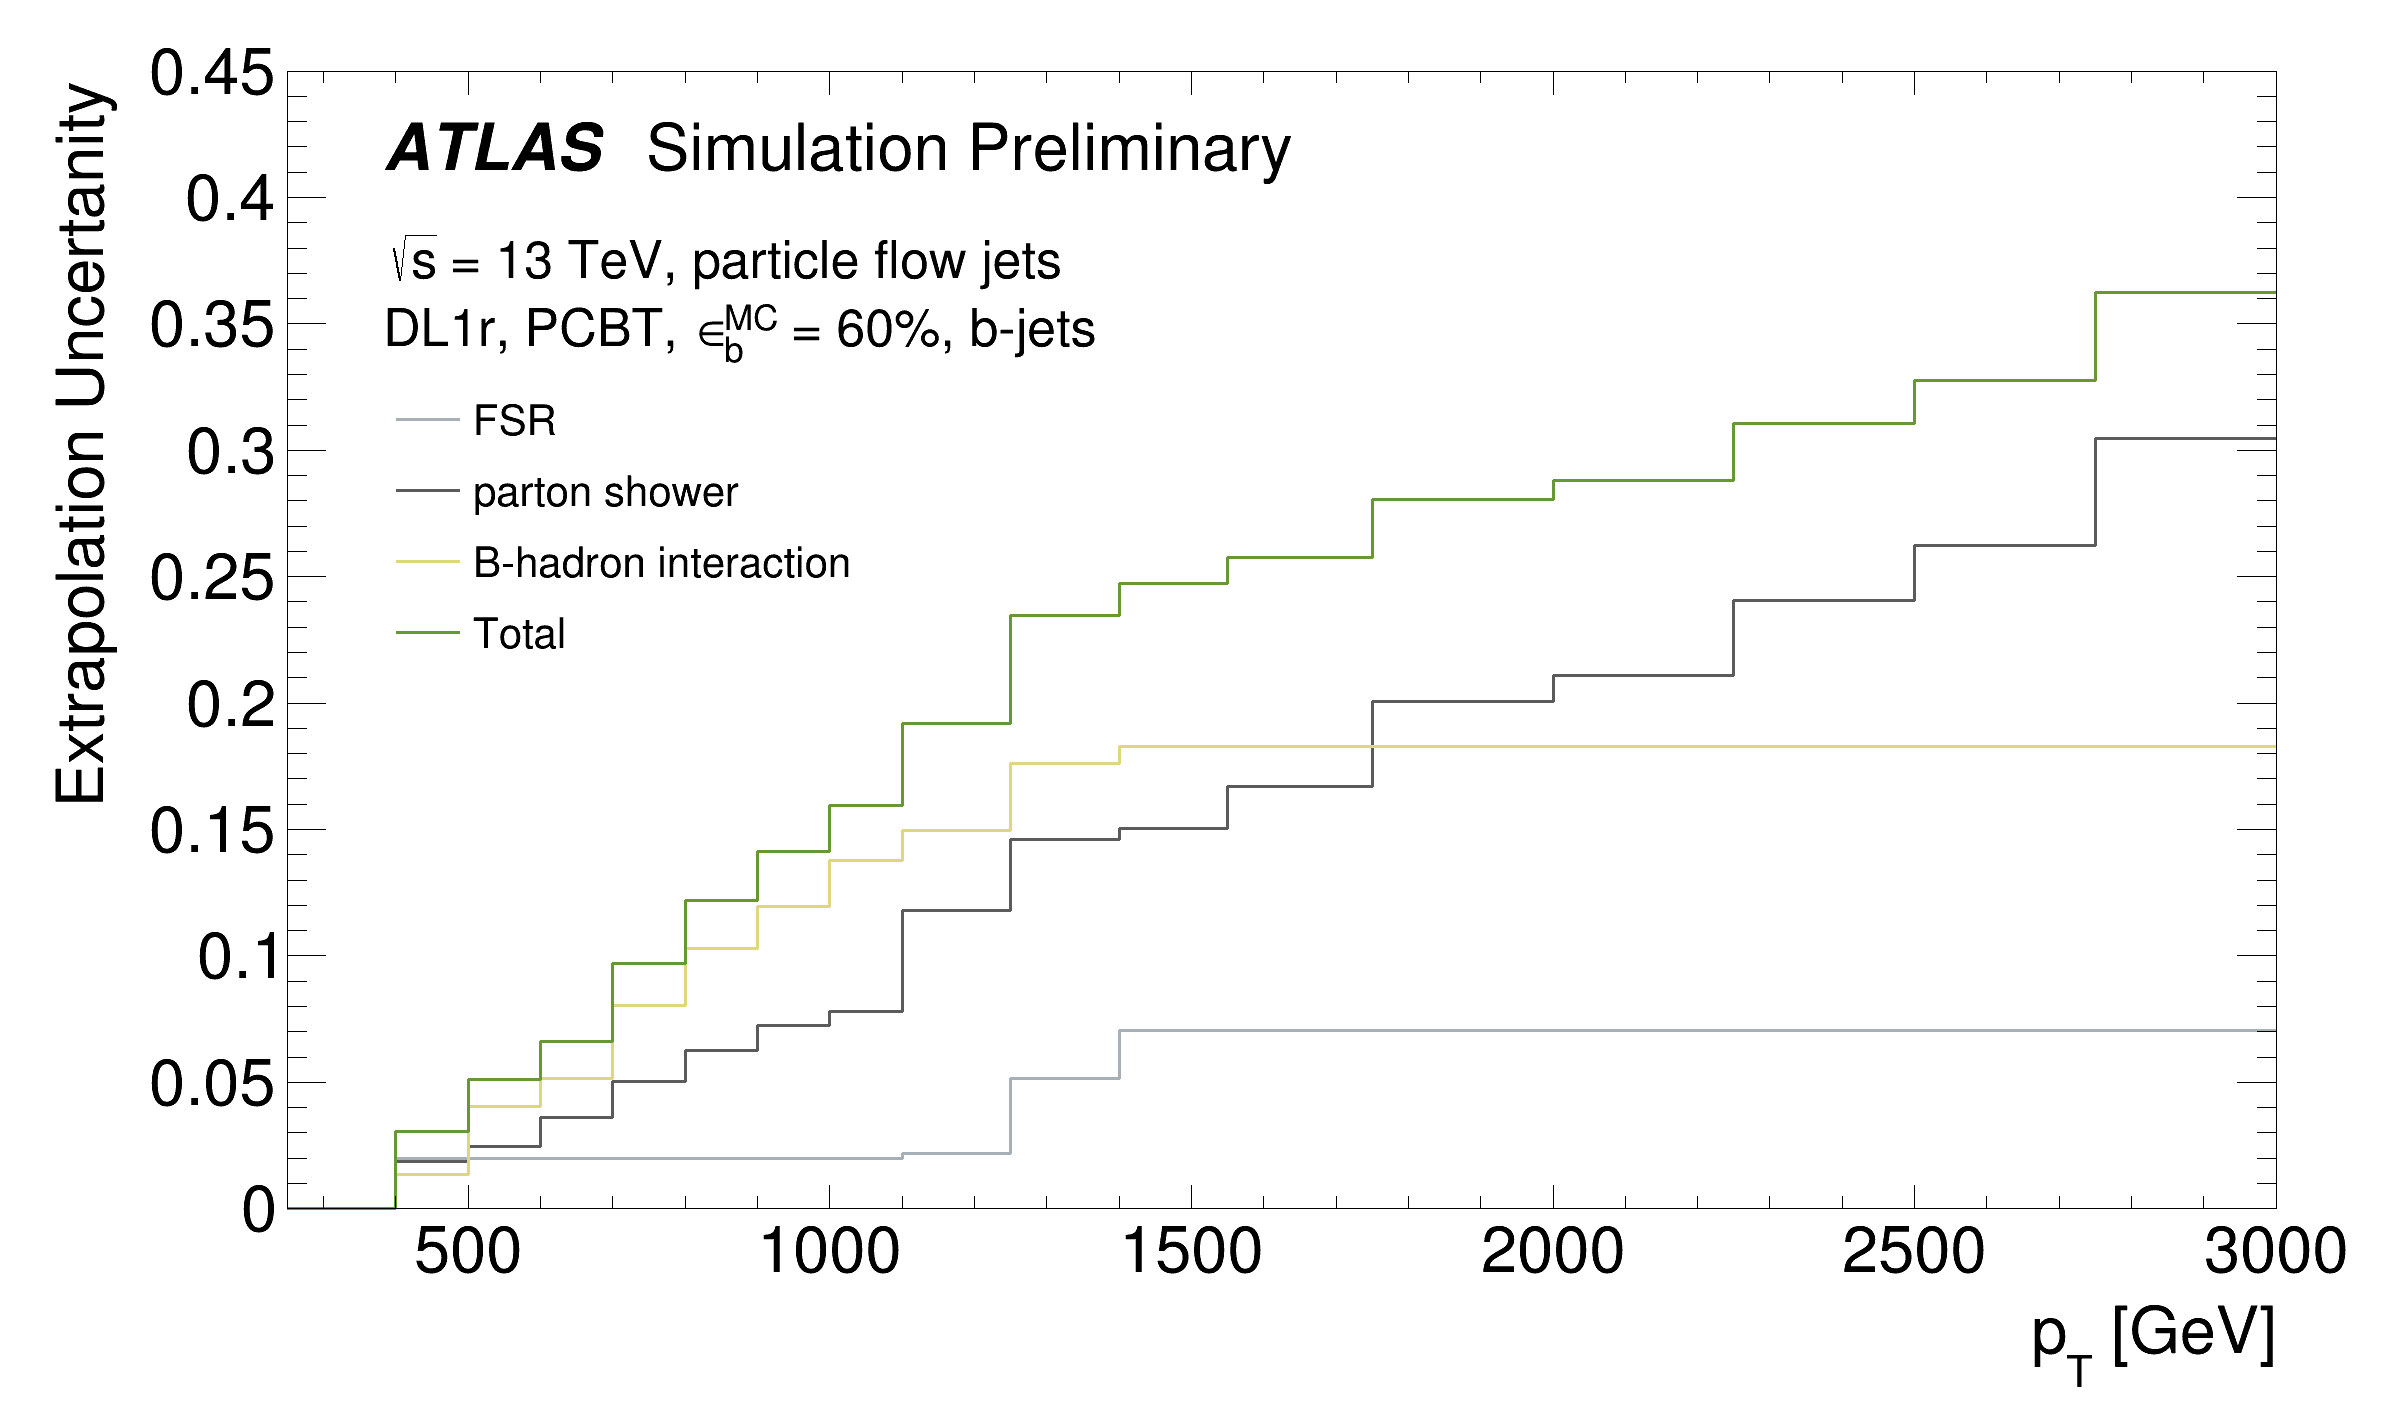
\includegraphics[scale=0.15]{figures/App_btag_highpt_extrap/modelling_important_extrap_uncs.png}
    \caption{The modeling extrapolation uncertainty containing: Final state radiation (FSR, light grey), B-hadron interaction (yellow), parton shower (dark grey) and the total combination of all modeling systematics (green).}
        \label{fig:modelextrap}
\end{figure}

\subsection{Global uncertainty}
As discussed in Section~\ref{sec:model} the modeling uncertainties are the dominant contributors for the extrapolation uncertainty. This is confirmed in Figures~\ref{fig:globalunc} and~\ref{fig:globalextrap}.
\begin{figure}[htbp]
    \centering
    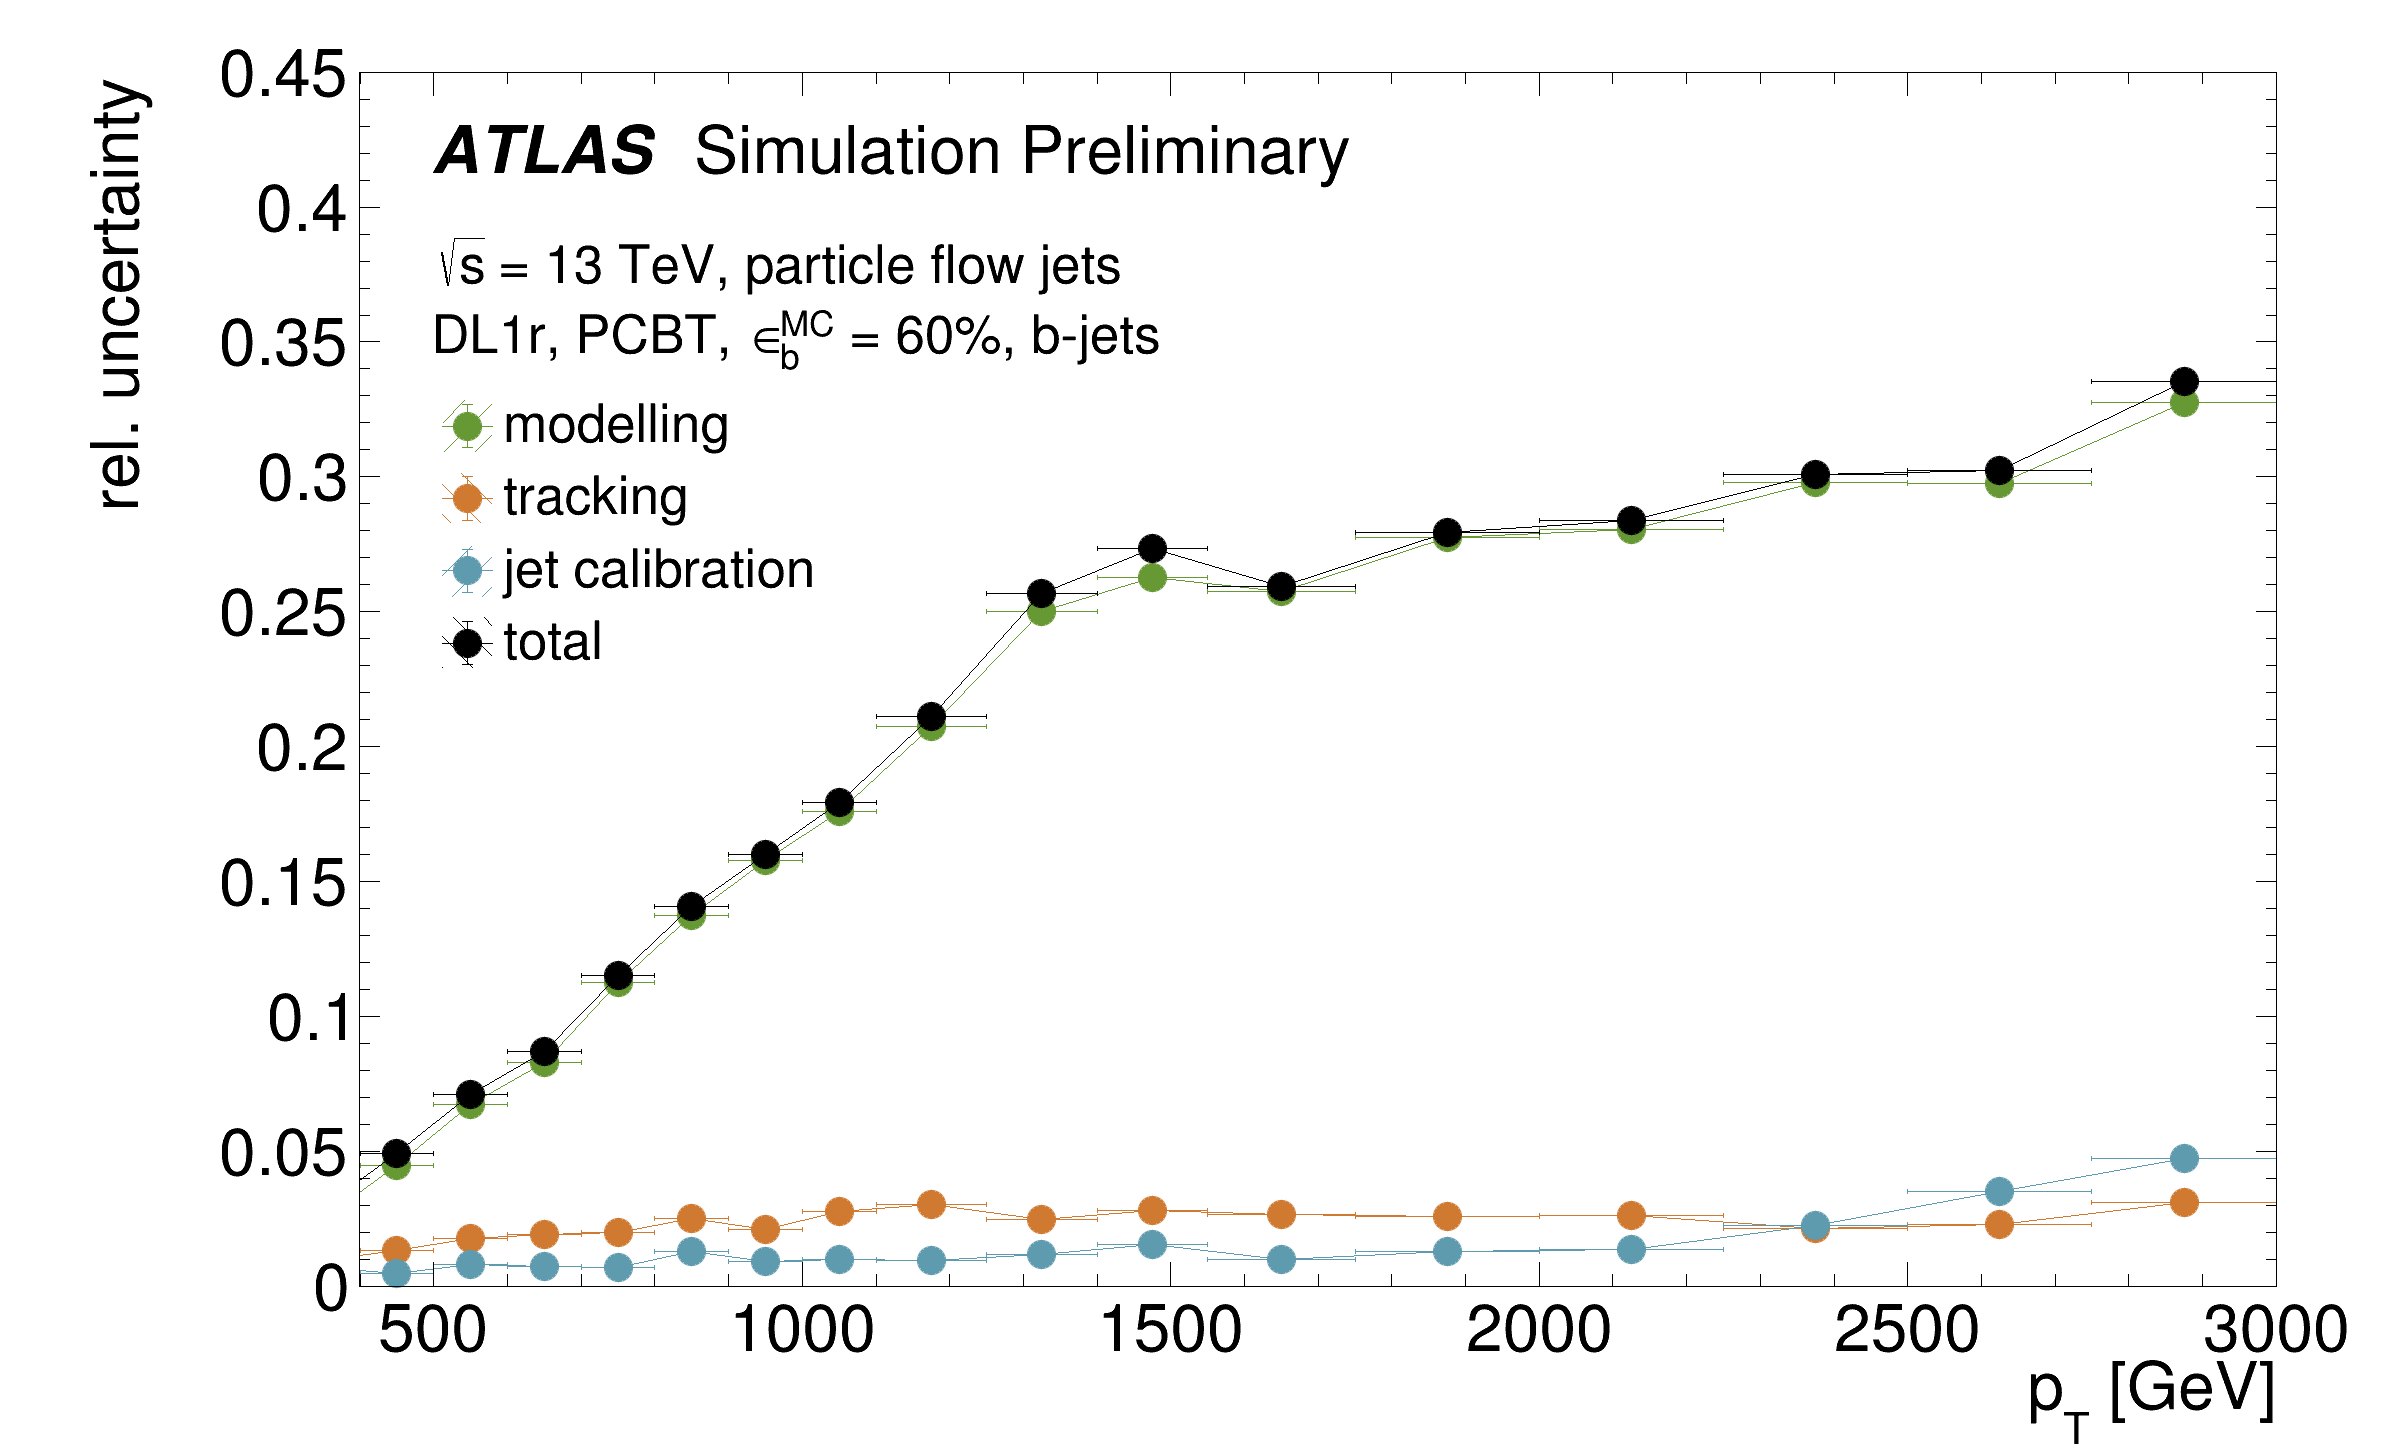
\includegraphics[scale=0.15]{figures/App_btag_highpt_extrap/global_uncs.png}
    \caption{The combination of all systematic totals to make the global uncertainty containing: modeling (Green), tracking (orange), jet calibration (blue) and the total (black). }
        \label{fig:globalunc}
\end{figure}


\begin{figure}[htbp]
    \centering
    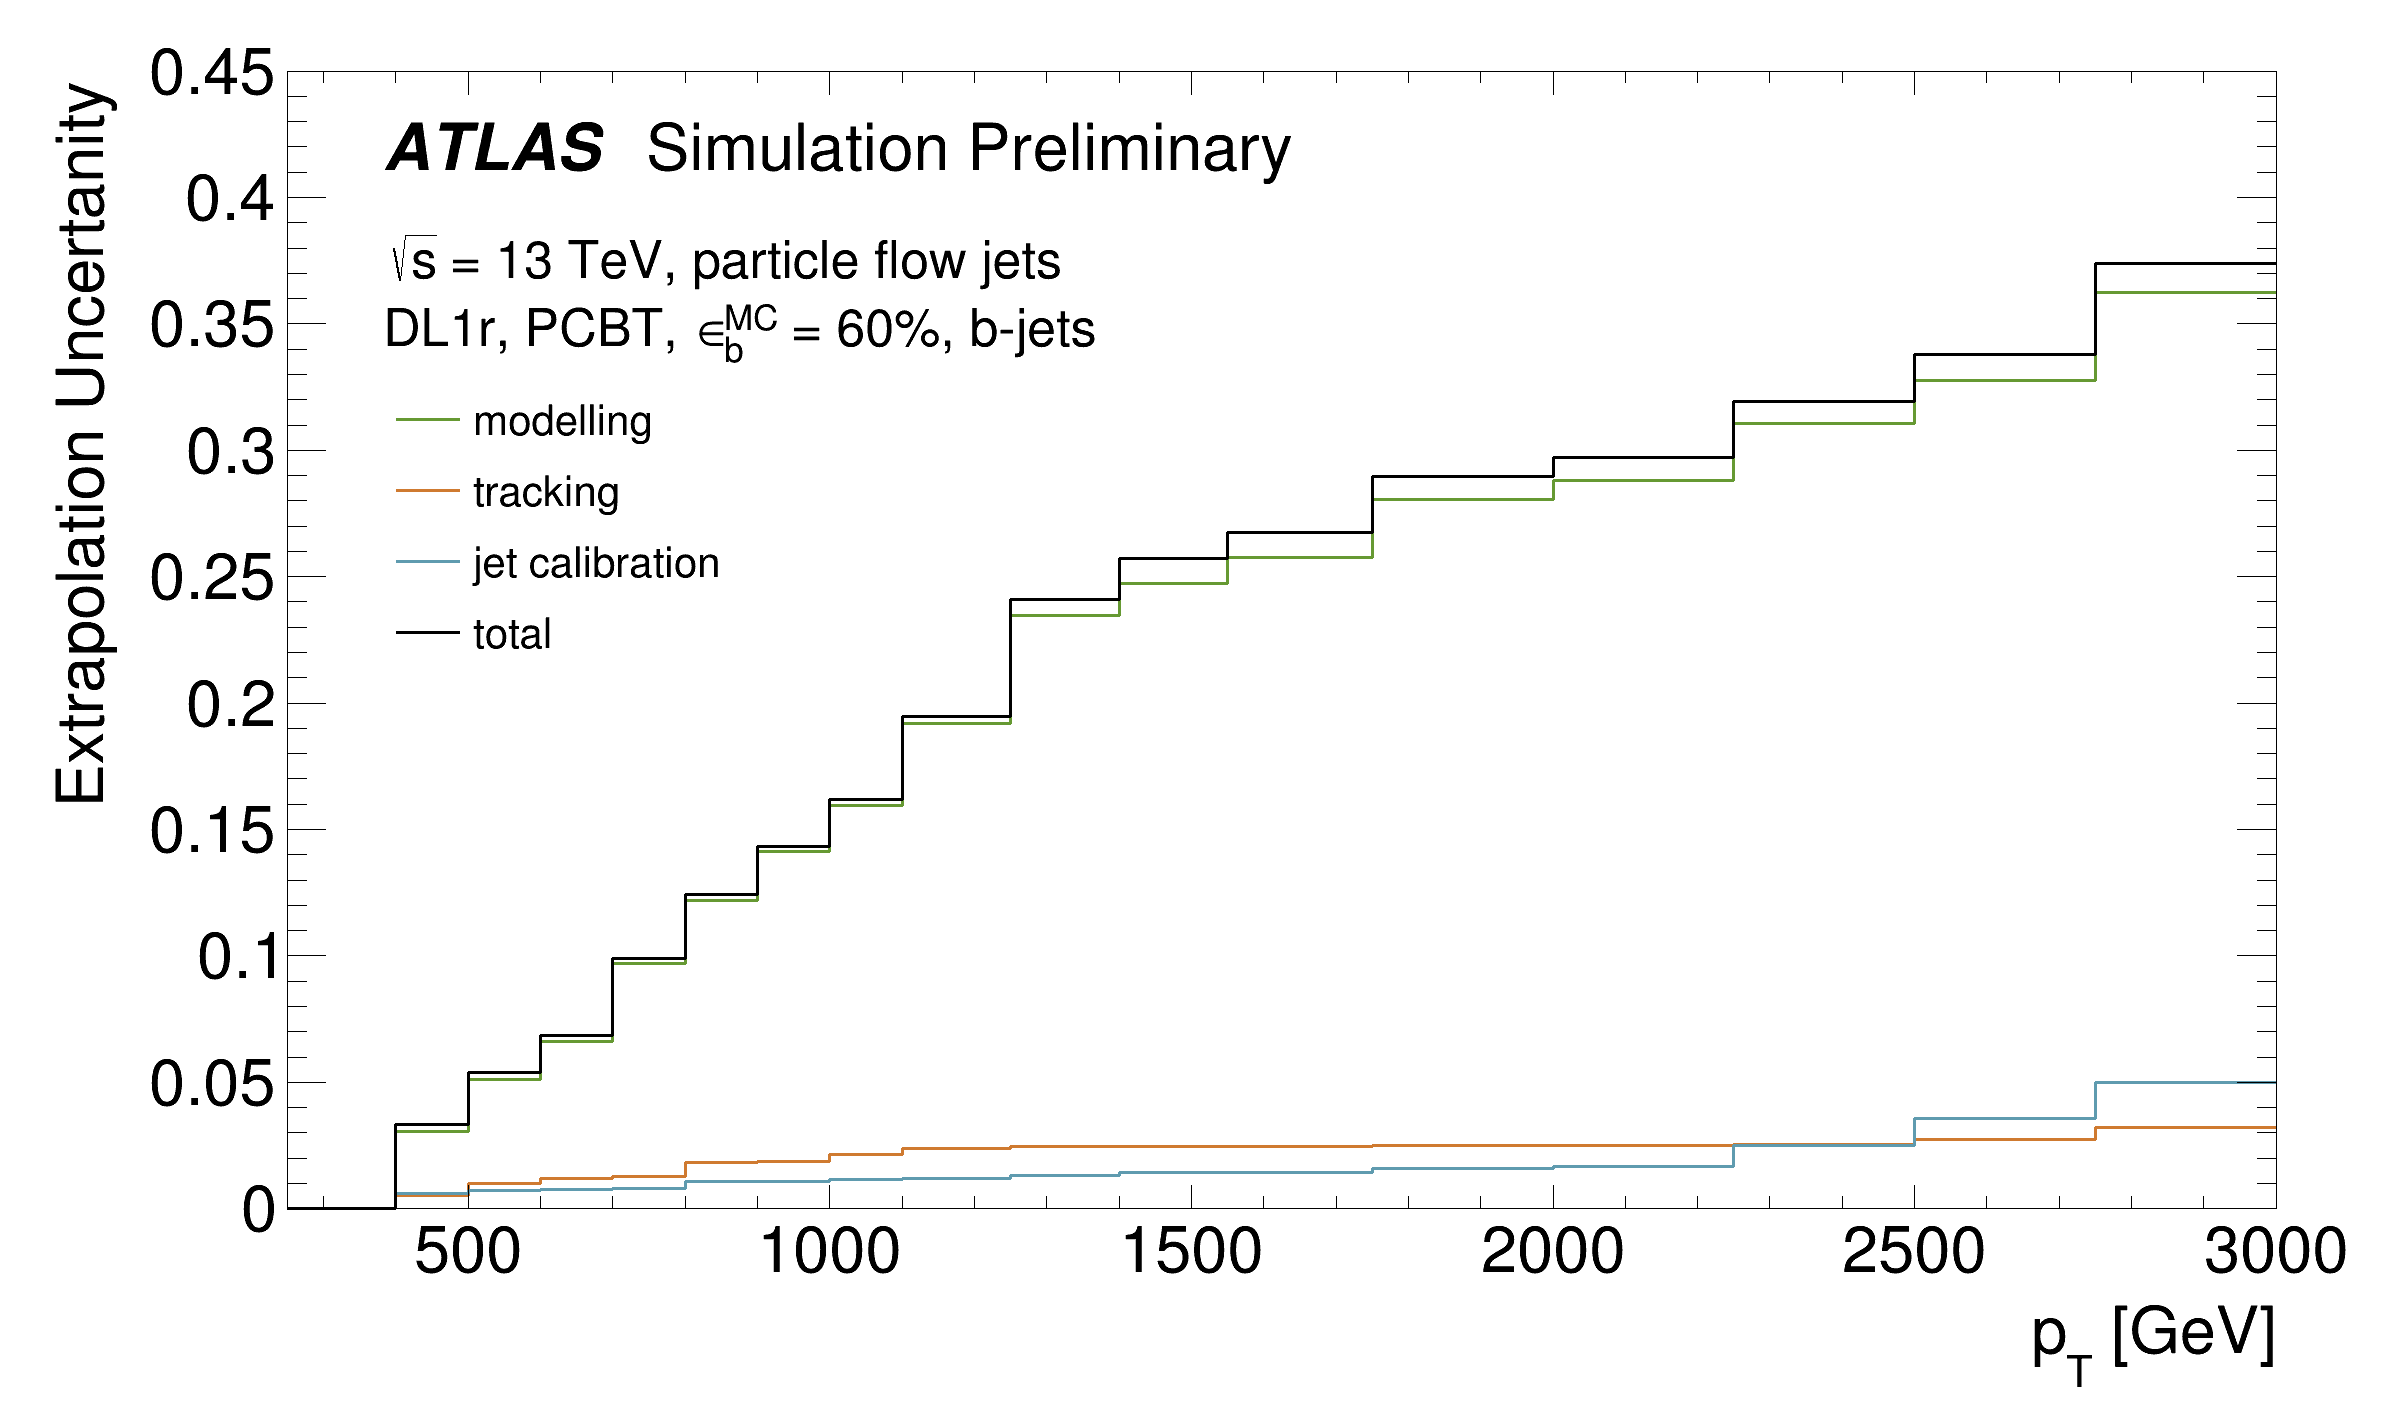
\includegraphics[scale=0.15]{figures/App_btag_highpt_extrap/global_extrap_uncs.png}
    \caption{The global extrapolation uncertainty containing: modeling (Green), tracking (orange), jet calibration (blue) and the total (black). }
        \label{fig:globalextrap}
\end{figure}


\section{Eigenvector Decomposition}
Folding the full set of extrapolated uncertainties into any analysis would result in a very bloated fit model, as we would have several nuisance parameters, per flavour of jet. To get around this issue, we can construct a matrix containing the contribution of each uncertainty per $p_T$ bin for one flavour of jet. Conducting an eigenvector (EV) decomposition on This matrix, resulting in a set of EVs were the leading EVs are encoded with the majority of the information from the initial matrix, selecting these leading EVs while pruning the rest folding these into our analysis would greatly reduce the bloat In our fit model while still capturing effects of the extrapolated uncertainties.
\\
Let us denote by $N$ the number of $p_T$ bins under consideration, and by $M$ the number of systematic uncertainty sources (e.g., tracking, pile-up, modelling, etc.) for one flavour of jet. The uncertainty contributions can be represented in a matrix
\begin{equation*}
\mathbf{U} \in \mathbb{R}^{N \times M},
\end{equation*}
where the element $u_{ik}$ represents the contribution of the $k$-th systematic source to the uncertainty in the $i$-th $p_T$ bin. Each column $\mathbf{u}_k$ of $\mathbf{U}$ encodes the shape of the $k$-th uncertainty across all bins.
\subsection*{Covariance Matrix Construction}
To study the correlations between the total uncertainties across $p_T$ bins, we construct the covariance matrix
\begin{equation*}
\mathbf{V} = \mathbf{U} \mathbf{U}^\top \in \mathbb{R}^{N \times N},
\end{equation*}
with components
\begin{equation*}
V_{ij} = \sum_{k=1}^{M} u_{ik} u_{jk}.
\end{equation*}
\subsection*{Eigenvector Decomposition}
We perform an eigenvector decomposition (EVD) on the covariance matrix $\mathbf{V}$:
\begin{equation*}
\mathbf{V} = \mathbf{Q} \boldsymbol{\Lambda} \mathbf{Q}^\top,
\end{equation*}
where:
\begin{itemize}
    \item $\mathbf{Q} = [\vec{v}_1, \vec{v}_2, \dots, \vec{v}_N]$ is an orthogonal matrix containing the eigenvectors of $\mathbf{V}$,
    \item $\boldsymbol{\Lambda} = \mathrm{diag}(\lambda_1^2, \dots, \lambda_N^2)$ is the diagonal matrix of eigenvalues.
\end{itemize}
Each eigenvector satisfies:
\begin{equation*}
\mathbf{V} \vec{v}_k = \lambda_k^2 \vec{v}_k,
\end{equation*}
and the orthonormality condition
\begin{equation*}
\vec{v}_i^\top \vec{v}_j = \delta_{ij}, \quad \Rightarrow \quad \mathbf{Q}^\top \mathbf{Q} = \mathbf{I}.
\end{equation*}
We then define a new matrix of eigenvector uncertainties:
\begin{equation*}
\tilde{\mathbf{U}} = \mathbf{Q} \boldsymbol{\Lambda}^{1/2},
\end{equation*}
with elements
\begin{equation*}
\tilde{u}_{ik} = \lambda_k v_{ik}.
\end{equation*}
\subsection*{Variance Preservation and Truncation}
The total variance in each bin $i$ is preserved under this transformation:
\begin{equation*}
\sum_{k=1}^{M} u_{ik}^2 = \sum_{k=1}^{N} \tilde{u}_{ik}^2 = V_{ii}.
\end{equation*}
Since the eigenvalues $\lambda_k^2$ are typically ordered such that $\lambda_1^2 \geq \lambda_2^2 \geq \cdots \geq \lambda_N^2$, most of the information is contained in the first few eigenvectors. Therefore, we can truncate the expansion by retaining only the leading $L < N$ components:
\begin{equation*}
\mathbf{V} \approx \sum_{k=1}^{L} \lambda_k^2 \vec{v}_k \vec{v}_k^\top.
\end{equation*}
This yields a reduced eigenvector uncertainty matrix:
\begin{equation*}
\tilde{\mathbf{U}}_{\text{reduced}} = \mathbf{Q}_{(L)} \boldsymbol{\Lambda}_{(L)}^{1/2},
\end{equation*}
where $\mathbf{Q}_{(L)}$ contains only the first $L$ eigenvectors, and $\boldsymbol{\Lambda}_{(L)}$ the corresponding eigenvalues.
\\
\\
In practice, this technique allows us to include only the dominant $L$ orthogonal modes as nuisance parameters in the analysis, dramatically reducing the dimensionality of the fit model while faithfully preserving the core features of the extrapolated uncertainty space.
\section{Post truncation validation}
After some discussion with FTAG the number of EVs to keep after truncation were settled on per flavour and are shown in table.~\ref{table:EV}. The question remains: if the number of EVs retained contain enough information to effectively encapsulate uncertainties evaluated thus far. \footnote{\href{https://twiki.cern.ch/twiki/bin/view/AtlasProtected/BTagCalibrationRecommendationsRelease21\#Recommendation_July_2023}{Link} to the twiki for the July 2023 recommendation.}.
\begin{center}
\begin{table}[h!]

    \centering
    \begin{tabular}{|c|c|}

    \hline
     Flavour&Number of eigenvectors
kept after truncation, $L$\\
    \hline
        $b$&4  \\
         $c$&2 \\
          $light$&4\\
         \hline
    \end{tabular}
    \caption{Number of eigenvectors kept after truncation per flavour.}
        \label{table:EV}
\end{table}
\end{center}
\\
\\
Figures \ref{fig:bev}, \ref{fig:cev} and \ref{fig:lev} show the full uncertainties for each $p_T$ bin, from immediately after calibration to 3 Tev, for each PCBT  WP, (black) and the uncertainties evaluated only using the truncated  set of EVs (red). As we see in Figure~\ref{fig:bev}, referring to $b$-jets, there is a max loss of information of $\approx$ 6\%. However, this is a 6\% loss of an overall uncertainty value of $\approx$ 5, leading to an overall precision loss of $<$ 0.3 in our final uncertainty value. Similarly, in Figure~\ref{fig:cev}, referring to $c$-jets, we see a maximum loss of information of $\approx$ 4\% of an original uncertainty value of 10 leading to an overall loss of 0.4. Finally, Figure~\ref{fig:lev}, referring to light-jets, we see a maximum information loss of $\approx$ 20\%. This is much larger than the previous flavours, however following the same logic as before, this is a $\approx$ 20\% loss of 16 resulting in an overall loss of 3.2 from our final uncertainty. The high level takeaway from this discussion is that: The bins immediately after calibration suffer the most form information loss in the truncated regime across all flavours. However, the magnitude of their information loss is minimal  due to the relative low value of the raw uncertainty, hence considered acceptable. 
\\
\\
After considering the information loss with the truncated set of EVs, the loss was deemed minor and FTAG accepted the recommendation to reduce the number of EVs detailed in \ref{table:EV}. With this recommendation in hand, FTAG propagated this work into the final CDI of release 21 and so any analysis using PFlow jets and the PCBT methods with high-$p_T$ regions could benefit form this extrapolation method and will provide more reliable flavour-tagging uncertainties past the calibration threshold.
\begin{figure}[h!]
    \centering
    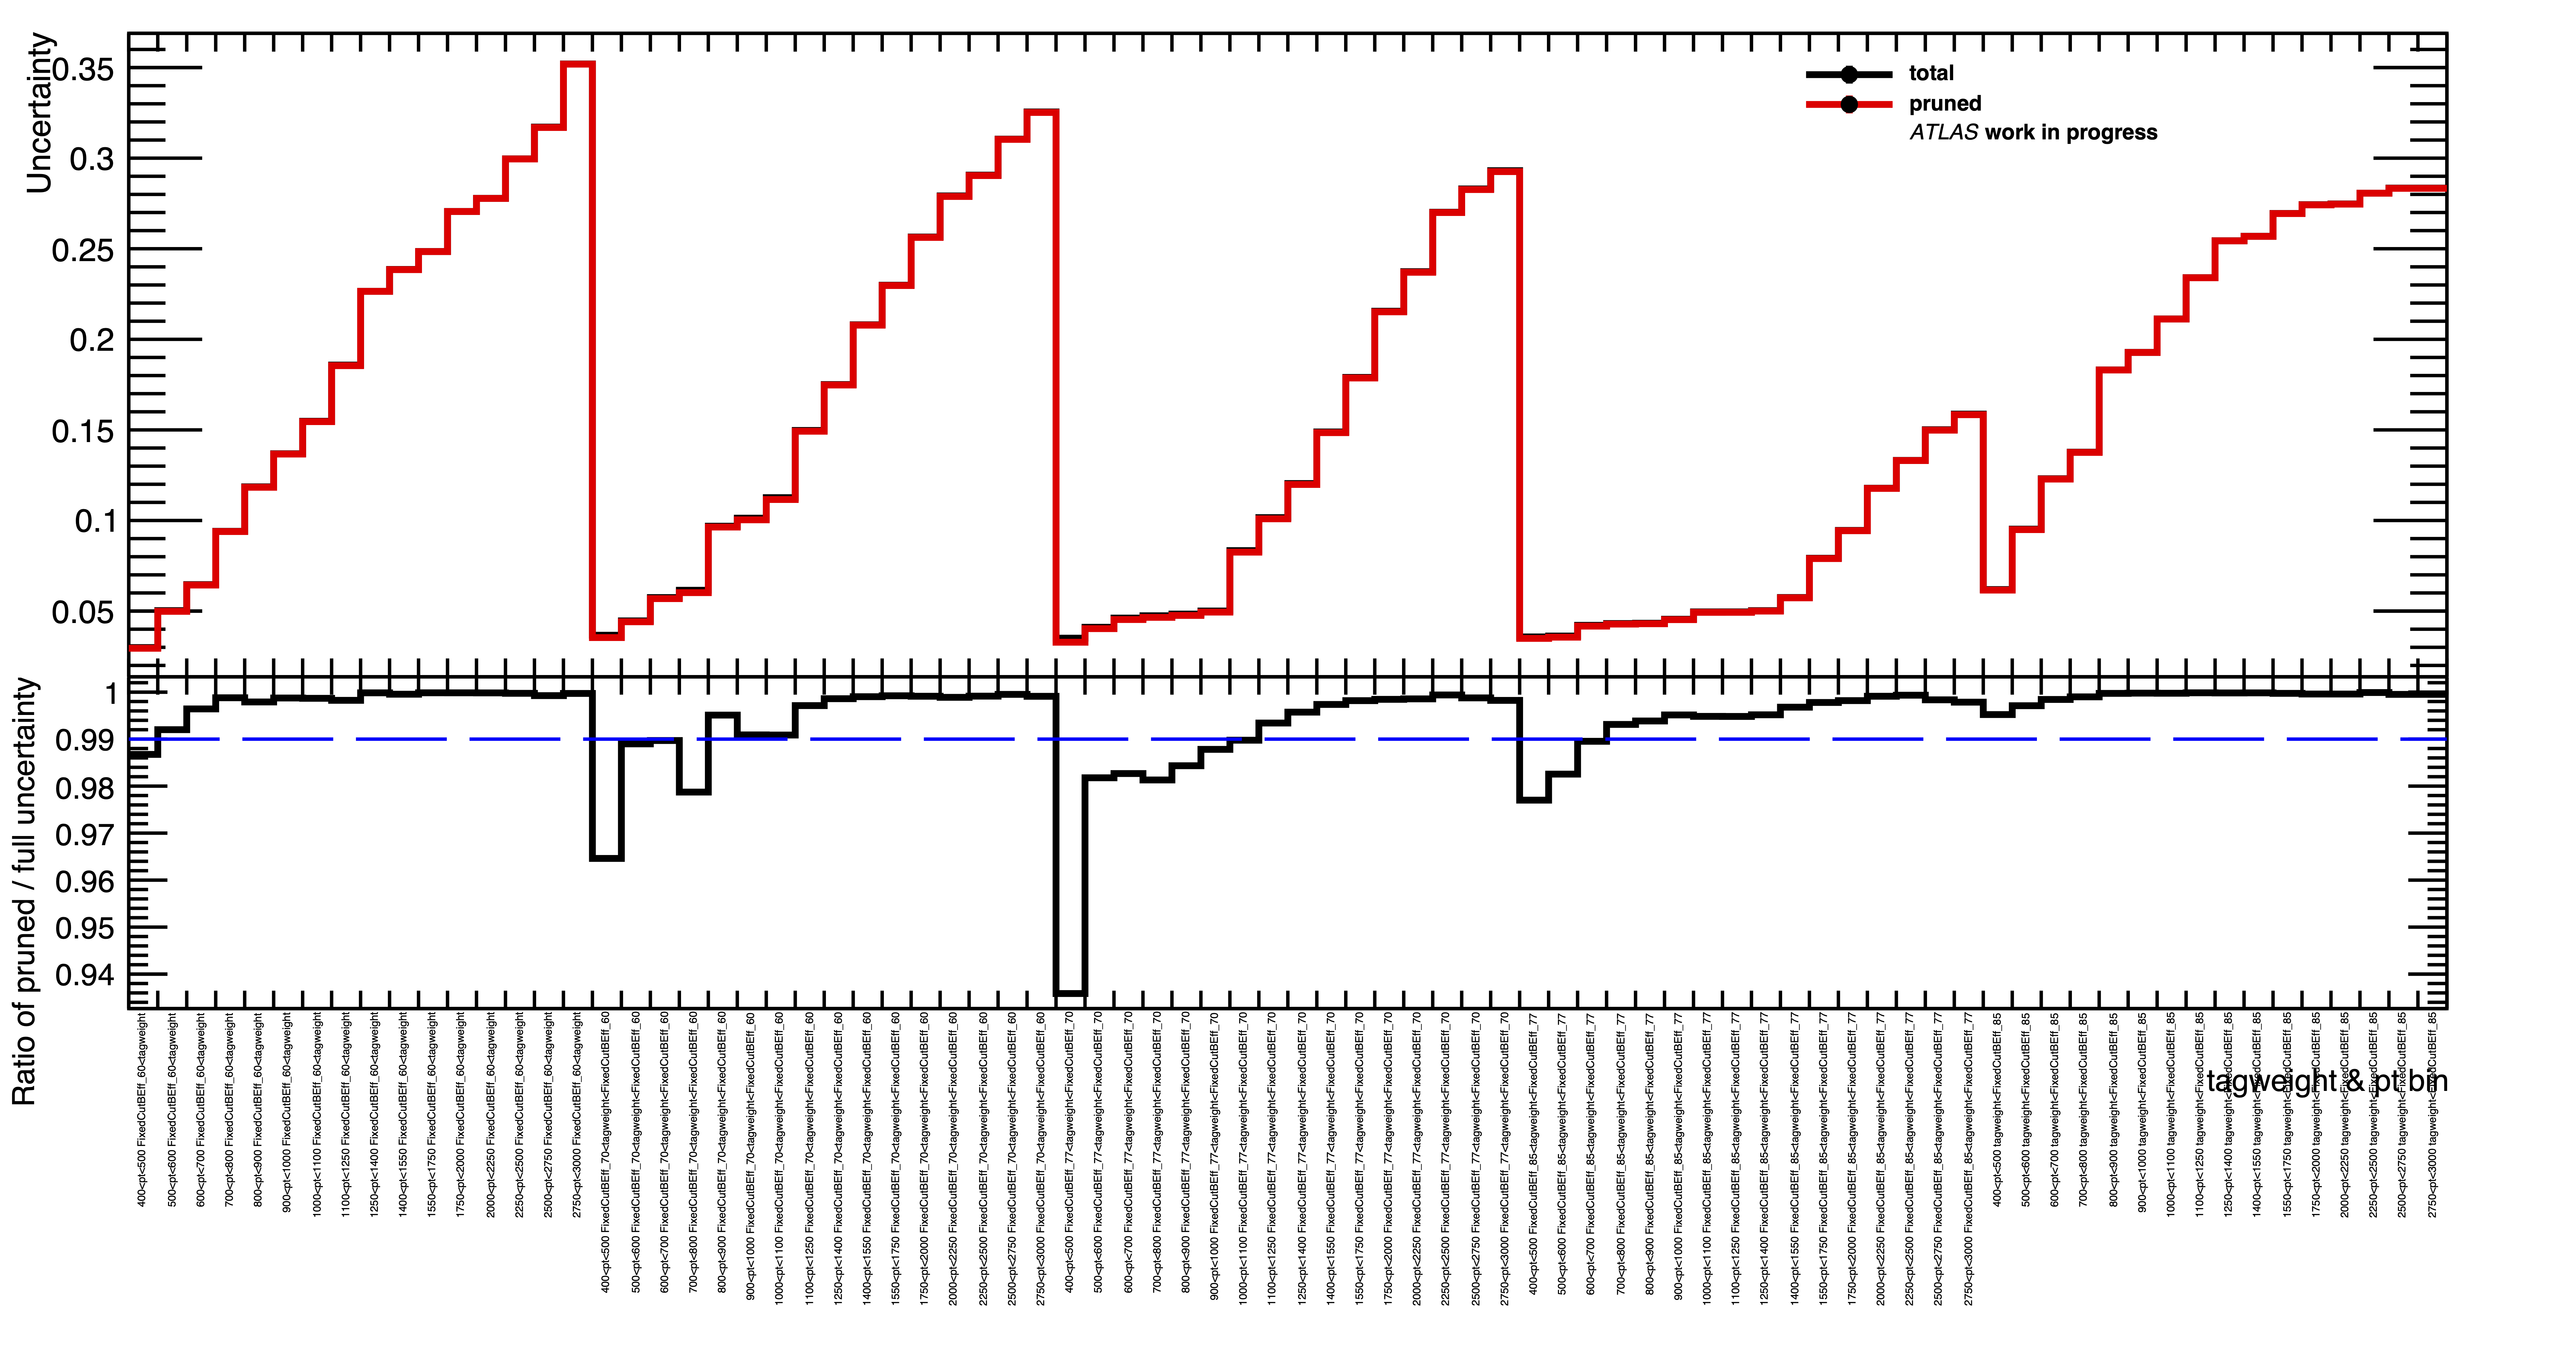
\includegraphics[scale=0.7]{figures/App_btag_highpt_extrap/ratio_vec_4_b.png}
    \caption{$b$-jets: The uncertainty for a particular $p_T$ bin after calibration and WP up to 3 TeV and the ratio of total (black) and pruned (red) eigenvectors, we keep 4 eigenvectors after the pruning stage. }
        \label{fig:bev}
\end{figure}
\begin{figure}[h!]
    \centering
    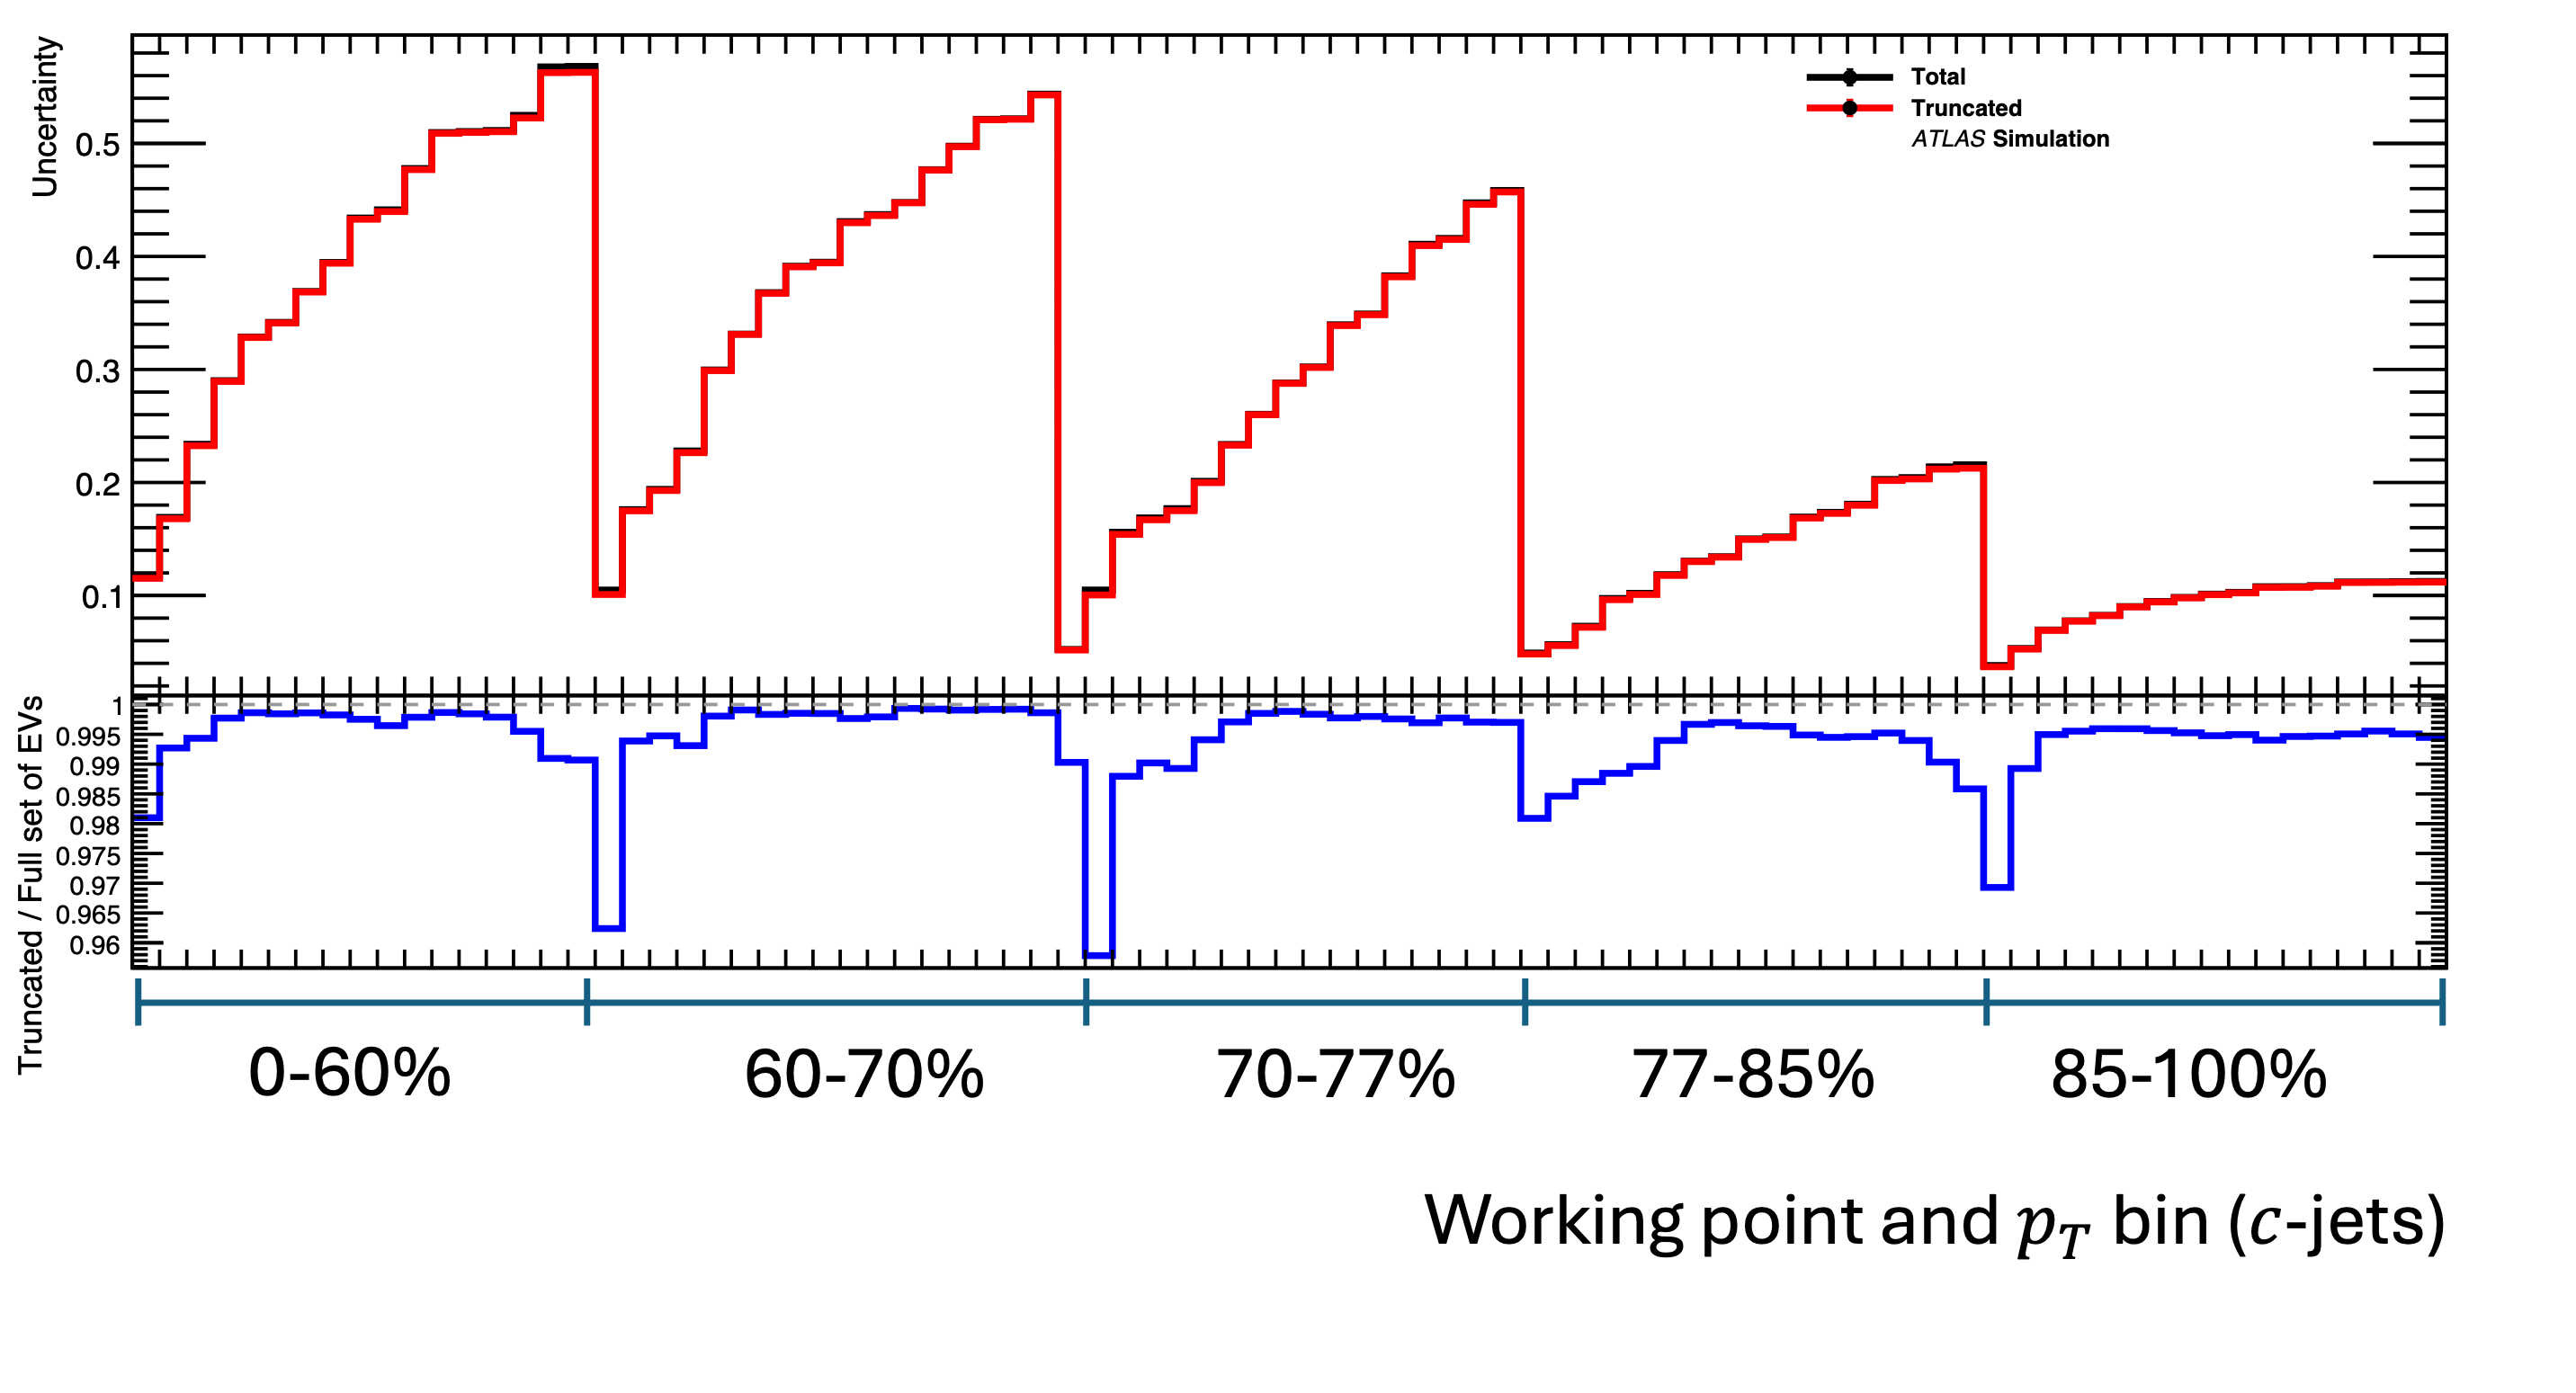
\includegraphics[scale=0.7]{figures/App_btag_highpt_extrap/ratio_vec_2_c.png}
    \caption{$c$-jets: The uncertainty for a particular $p_T$ bin  after calibration and WP up to 3 TeV and the ratio of total (black) and pruned (red) eigenvectors, we keep 2 eigenvectors after the pruning stage. }
        \label{fig:cev}
\end{figure}
\begin{figure}[h!]
    \centering
    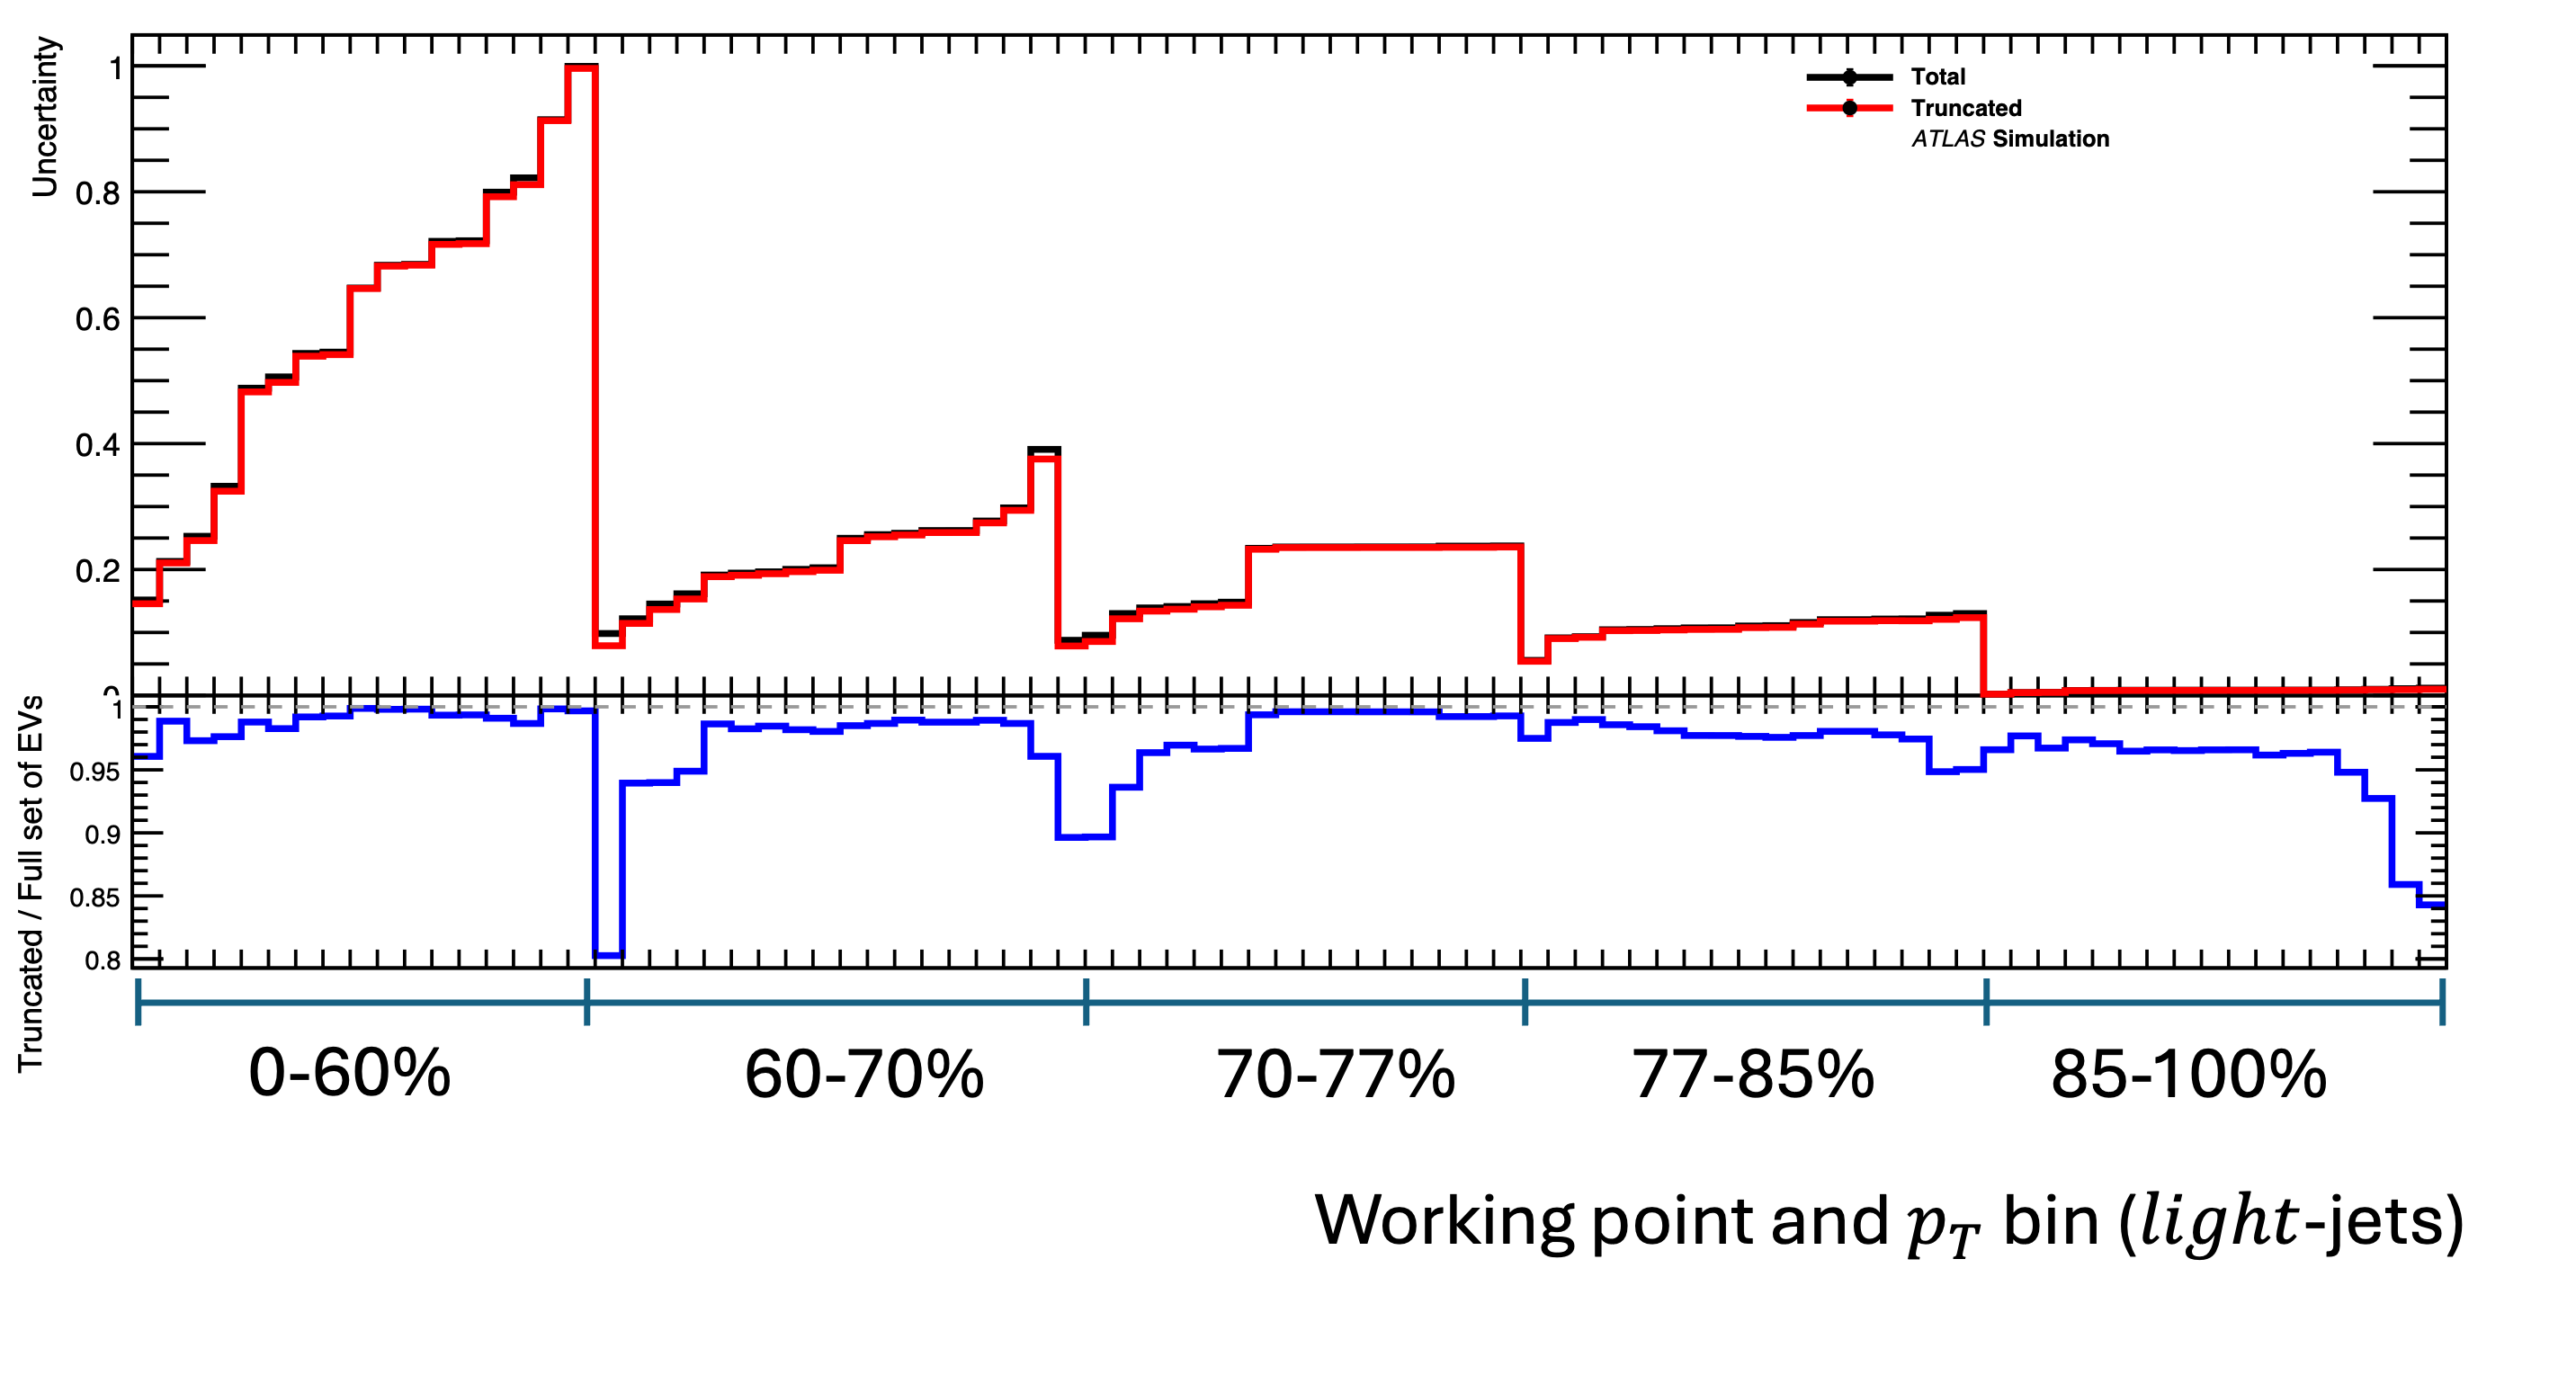
\includegraphics[scale=0.7]{figures/App_btag_highpt_extrap/ratio_vec_4_l.png}
    \caption{$light$-jets: The uncertainty for a particular $p_T$ bin  after calibration and WP up to 3 TeV and the ratio of total (black) and pruned (red) eigenvectors, we keep 4 eigenvectors after the pruning stage. }
        \label{fig:lev}
\end{figure}